\documentclass[twoside]{book}

% Packages required by doxygen
\usepackage{fixltx2e}
\usepackage{calc}
\usepackage{doxygen}
\usepackage[export]{adjustbox} % also loads graphicx
\usepackage{graphicx}
\usepackage[utf8]{inputenc}
\usepackage{makeidx}
\usepackage{multicol}
\usepackage{multirow}
\PassOptionsToPackage{warn}{textcomp}
\usepackage{textcomp}
\usepackage[nointegrals]{wasysym}
\usepackage[table]{xcolor}

% Font selection
\usepackage[T1]{fontenc}
\usepackage[scaled=.90]{helvet}
\usepackage{courier}
\usepackage{amssymb}
\usepackage{sectsty}
\renewcommand{\familydefault}{\sfdefault}
\allsectionsfont{%
  \fontseries{bc}\selectfont%
  \color{darkgray}%
}
\renewcommand{\DoxyLabelFont}{%
  \fontseries{bc}\selectfont%
  \color{darkgray}%
}
\newcommand{\+}{\discretionary{\mbox{\scriptsize$\hookleftarrow$}}{}{}}

% Page & text layout
\usepackage{geometry}
\geometry{%
  a4paper,%
  top=2.5cm,%
  bottom=2.5cm,%
  left=2.5cm,%
  right=2.5cm%
}
\tolerance=750
\hfuzz=15pt
\hbadness=750
\setlength{\emergencystretch}{15pt}
\setlength{\parindent}{0cm}
\setlength{\parskip}{3ex plus 2ex minus 2ex}
\makeatletter
\renewcommand{\paragraph}{%
  \@startsection{paragraph}{4}{0ex}{-1.0ex}{1.0ex}{%
    \normalfont\normalsize\bfseries\SS@parafont%
  }%
}
\renewcommand{\subparagraph}{%
  \@startsection{subparagraph}{5}{0ex}{-1.0ex}{1.0ex}{%
    \normalfont\normalsize\bfseries\SS@subparafont%
  }%
}
\makeatother

% Headers & footers
\usepackage{fancyhdr}
\pagestyle{fancyplain}
\fancyhead[LE]{\fancyplain{}{\bfseries\thepage}}
\fancyhead[CE]{\fancyplain{}{}}
\fancyhead[RE]{\fancyplain{}{\bfseries\leftmark}}
\fancyhead[LO]{\fancyplain{}{\bfseries\rightmark}}
\fancyhead[CO]{\fancyplain{}{}}
\fancyhead[RO]{\fancyplain{}{\bfseries\thepage}}
\fancyfoot[LE]{\fancyplain{}{}}
\fancyfoot[CE]{\fancyplain{}{}}
\fancyfoot[RE]{\fancyplain{}{\bfseries\scriptsize Generated by Doxygen }}
\fancyfoot[LO]{\fancyplain{}{\bfseries\scriptsize Generated by Doxygen }}
\fancyfoot[CO]{\fancyplain{}{}}
\fancyfoot[RO]{\fancyplain{}{}}
\renewcommand{\footrulewidth}{0.4pt}
\renewcommand{\chaptermark}[1]{%
  \markboth{#1}{}%
}
\renewcommand{\sectionmark}[1]{%
  \markright{\thesection\ #1}%
}

% Indices & bibliography
\usepackage{natbib}
\usepackage[titles]{tocloft}
\setcounter{tocdepth}{3}
\setcounter{secnumdepth}{5}
\makeindex

% Hyperlinks (required, but should be loaded last)
\usepackage{ifpdf}
\ifpdf
  \usepackage[pdftex,pagebackref=true]{hyperref}
\else
  \usepackage[ps2pdf,pagebackref=true]{hyperref}
\fi
\hypersetup{%
  colorlinks=true,%
  linkcolor=blue,%
  citecolor=blue,%
  unicode%
}

% Custom commands
\newcommand{\clearemptydoublepage}{%
  \newpage{\pagestyle{empty}\cleardoublepage}%
}

\usepackage{caption}
\captionsetup{labelsep=space,justification=centering,font={bf},singlelinecheck=off,skip=4pt,position=top}

%===== C O N T E N T S =====

\begin{document}

% Titlepage & ToC
\hypersetup{pageanchor=false,
             bookmarksnumbered=true,
             pdfencoding=unicode
            }
\pagenumbering{alph}
\begin{titlepage}
\vspace*{7cm}
\begin{center}%
{\Large Library\+Astrodynamics \\[1ex]\large 2018.\+06.\+16 }\\
\vspace*{1cm}
{\large Generated by Doxygen 1.8.13}\\
\end{center}
\end{titlepage}
\clearemptydoublepage
\pagenumbering{roman}
\tableofcontents
\clearemptydoublepage
\pagenumbering{arabic}
\hypersetup{pageanchor=true}

%--- Begin generated contents ---
\chapter{Library \+:\+: Astrodynamics}
\label{index}\hypertarget{index}{}Structure

\href{https://github.com/open-space-collective/open-space-toolkit-astrodynamics/actions/workflows/build-test.yml}{\tt } \href{https://codecov.io/gh/open-space-collective/open-space-toolkit-astrodynamics}{\tt } \href{https://open-space-collective.github.io/open-space-toolkit-astrodynamics}{\tt } \href{https://badge.fury.io/gh/open-space-collective%2Fopen-space-toolkit-astrodynamics}{\tt } \href{https://badge.fury.io/py/open-space-toolkit-astrodynamics}{\tt } \href{https://opensource.org/licenses/Apache-2.0}{\tt }

Orbit, attitude, access.



\subsection*{Getting Started}

Want to get started? This is the simplest and quickest way\+:

\href{https://mybinder.org/v2/gh/open-space-collective/open-space-toolkit/main?urlpath=lab/tree/notebooks}{\tt }

{\itshape Nothing to download or install! This will automatically start a \href{https://jupyterlab.readthedocs.io/en/stable/}{\tt Jupyter\+Lab} environment in your browser with Open Space Toolkit libraries and example notebooks ready to use.}

\subsubsection*{Alternatives}

\paragraph*{Docker Images}

\href{https://www.docker.com/}{\tt Docker} must be installed on your system.

\subparagraph*{i\+Python}

The following command will start an \href{https://ipython.org/}{\tt i\+Python} shell within a container where the O\+S\+Tk components are already installed\+:


\begin{DoxyCode}
docker run -it openspacecollective/open-space-toolkit-astrodynamics-python
\end{DoxyCode}


Once the shell is up and running, playing with it is easy\+:


\begin{DoxyCode}
\textcolor{keyword}{from} ostk.physics \textcolor{keyword}{import} Environment
\textcolor{keyword}{from} ostk.physics.time \textcolor{keyword}{import} Instant
\textcolor{keyword}{from} ostk.astrodynamics.trajectory \textcolor{keyword}{import} Orbit
\textcolor{keyword}{from} ostk.astrodynamics.trajectory.orbit.models \textcolor{keyword}{import} SGP4
\textcolor{keyword}{from} ostk.astrodynamics.trajectory.orbit.models.sgp4 \textcolor{keyword}{import} TLE

tle = TLE(
    \textcolor{stringliteral}{'1 25544U 98067A   18231.17878740  .00000187  00000-0  10196-4 0  9994'},
    \textcolor{stringliteral}{'2 25544  51.6447  64.7824 0005971  73.1467  36.4366 15.53848234128316'}
)  \textcolor{comment}{# Construct Two-Line Element set}

earth = Environment.default().access\_celestial\_object\_with\_name(\textcolor{stringliteral}{'Earth'})  \textcolor{comment}{# Access Earth model}

orbit = Orbit(SGP4(tle), earth)  \textcolor{comment}{# Construct orbit using SGP4 model}

orbit.get\_state\_at(Instant.now())  \textcolor{comment}{# Compute and display current satellite state (position, velocity)}
\end{DoxyCode}


By default, O\+S\+Tk fetches the ephemeris from J\+PL, Earth Orientation Parameters (E\+OP) and leap second count from I\+E\+RS.

As a result, when running O\+S\+Tk for the first time, it may take a minute to fetch all the necessary data.

{\itshape Tip\+: Use tab for auto-\/completion!}

\subparagraph*{Jupyter\+Lab}

The following command will start a \href{https://jupyterlab.readthedocs.io/en/stable/}{\tt Jupyter\+Lab} server within a container where the O\+S\+Tk components are already installed\+:


\begin{DoxyCode}
docker run --publish=8888:8888 openspacecollective/open-space-toolkit-astrodynamics-jupyter
\end{DoxyCode}


Once the container is running, access \href{http://localhost:8888/lab}{\tt http\+://localhost\+:8888/lab} and create a Python 3 Notebook.

\subsection*{Installation}

\subsubsection*{C++}

The binary packages are hosted using \href{https://github.com/open-space-collective/open-space-toolkit-astrodynamics/releases}{\tt Git\+Hub Releases}\+:


\begin{DoxyItemize}
\item Runtime libraries\+: {\ttfamily open-\/space-\/toolkit-\/astrodynamics-\/\+X.\+Y.\+Z-\/1.\+x86\+\_\+64-\/runtime}
\item C++ headers\+: {\ttfamily open-\/space-\/toolkit-\/astrodynamics-\/\+X.\+Y.\+Z-\/1.\+x86\+\_\+64-\/devel}
\item Python bindings\+: {\ttfamily open-\/space-\/toolkit-\/astrodynamics-\/\+X.\+Y.\+Z-\/1.\+x86\+\_\+64-\/python}
\end{DoxyItemize}

\paragraph*{Debian / Ubuntu}

After downloading the relevant {\ttfamily .deb} binary packages, install\+:


\begin{DoxyCode}
apt install open-space-toolkit-astrodynamics-*.deb
\end{DoxyCode}


\paragraph*{Fedora / Cent\+OS}

After downloading the relevant {\ttfamily .rpm} binary packages, install\+:


\begin{DoxyCode}
dnf install open-space-toolkit-astrodynamics-*.rpm
\end{DoxyCode}


\subsubsection*{Python}

Install from \href{https://pypi.org/project/open-space-toolkit-astrodynamics/}{\tt Py\+PI}\+:


\begin{DoxyCode}
pip install open-space-toolkit-astrodynamics
\end{DoxyCode}


\subsection*{Documentation}

Documentation is available here\+:


\begin{DoxyItemize}
\item \href{https://open-space-collective.github.io/open-space-toolkit-astrodynamics}{\tt C++}
\item \href{./bindings/python/docs}{\tt Python}
\end{DoxyItemize}

$<$details$>$

The library exhibits the following detailed and descriptive structure\+:


\begin{DoxyCode}
├── NumericalSolver
├── Trajectory
│   ├── State
│   ├── Orbit
│   │   ├── Models
│   │   │   ├── Kepler
│   │   │   │   └── Classical Orbital Elements (COE)
│   │   │   ├── SGP4
│   │   │   │   └── Two-Line Element \textcolor{keyword}{set} (TLE)
│   │   │   ├── Tabulated (input csv)
│   │   │   └── Propagated (numerical integration)
│   │   ├── Pass
|   |   └── Messages
|   |       └── SpaceX
|   |           └── OPM
│   ├── Models
│   |   ├── Static
│   |   └── Tabulated
│   └── Propagator
├── Flight
│   ├── Profile
|   |    ├── Models
│   |    |   ├── Transform
│   |    |   └── Tabulated
│   |    └── State
│   └── System
|        ├── SatelliteSystem
|        └── Dynamics
|            └── SatelliteDynamics
├── Access
|   └── Generator
└── Conjunction
    └── Messages
        └── CCSDS
            └── CDM
\end{DoxyCode}


$<$/details$>$

\subsection*{Tutorials}

Tutorials are available here\+:


\begin{DoxyItemize}
\item \href{./tutorials/cpp}{\tt C++}
\item \href{./tutorials/python}{\tt Python}
\end{DoxyItemize}

\subsection*{Setup}

\subsubsection*{Development Environment}

Using \href{https://www.docker.com}{\tt Docker} for development is recommended, to simplify the installation of the necessary build tools and dependencies. Instructions on how to install Docker are available \href{https://docs.docker.com/install/}{\tt here}.

To start the development environment\+:


\begin{DoxyCode}
make start-development
\end{DoxyCode}


This will\+:


\begin{DoxyEnumerate}
\item Build the {\ttfamily openspacecollective/open-\/space-\/toolkit-\/astrodynamics-\/development} Docker image.
\item Create a development environment container with local source files and helper scripts mounted.
\item Start a {\ttfamily bash} shell from the {\ttfamily ./build} working directory.
\end{DoxyEnumerate}

If installing Docker is not an option, you can manually install the development tools (G\+CC, C\+Make) and all required dependencies, by following a procedure similar to the one described in the \href{./docker/development/Dockerfile}{\tt Development Dockerfile}.

\subsubsection*{Build}

From the {\ttfamily ./build} directory\+:


\begin{DoxyCode}
cmake ..
make
\end{DoxyCode}


{\itshape Tip\+: {\ttfamily helpers/build.\+sh} simplifies building from within the development environment.}

\subsubsection*{Test}

To start a container to build and run the tests\+:


\begin{DoxyCode}
make test
\end{DoxyCode}


Or to run them manually\+:


\begin{DoxyCode}
./bin/open-space-toolkit-astrodynamics.test
\end{DoxyCode}


{\itshape Tip\+: {\ttfamily helpers/test.\+sh} simplifies running tests from within the development environment.}

\subsection*{Dependencies}

\tabulinesep=1mm
\begin{longtabu} spread 0pt [c]{*{4}{|X[-1]}|}
\hline
\rowcolor{\tableheadbgcolor}\textbf{ Name }&\textbf{ Version }&\textbf{ License }&\textbf{ Link  }\\\cline{1-4}
\endfirsthead
\hline
\endfoot
\hline
\rowcolor{\tableheadbgcolor}\textbf{ Name }&\textbf{ Version }&\textbf{ License }&\textbf{ Link  }\\\cline{1-4}
\endhead
Pybind11 &{\ttfamily 2.\+10.\+1} &B\+S\+D-\/3-\/\+Clause &\href{https://github.com/pybind/pybind11}{\tt github.\+com/pybind/pybind11} \\\cline{1-4}
ordered-\/map &{\ttfamily 0.\+6.\+0} &M\+IT &\href{https://github.com/Tessil/ordered-map}{\tt github.\+com/\+Tessil/ordered-\/map} \\\cline{1-4}
Eigen &{\ttfamily 3.\+3.\+7} &M\+P\+L2 &\href{http://eigen.tuxfamily.org/index.php}{\tt eigen.\+tuxfamily.\+org} \\\cline{1-4}
S\+G\+P4 &{\ttfamily 6a448b4} &Apache License 2.\+0 &\href{https://github.com/dnwrnr/sgp4}{\tt github.\+com/dnwrnr/sgp4} \\\cline{1-4}
N\+Lopt &{\ttfamily 2.\+5.\+0} &L\+G\+PL &\href{https://github.com/stevengj/nlopt}{\tt github.\+com/stevengj/nlopt} \\\cline{1-4}
Core &{\ttfamily main} &Apache License 2.\+0 &\href{https://github.com/open-space-collective/open-space-toolkit-core}{\tt github.\+com/open-\/space-\/collective/open-\/space-\/toolkit-\/core} \\\cline{1-4}
I/O &{\ttfamily main} &Apache License 2.\+0 &\href{https://github.com/open-space-collective/open-space-toolkit-io}{\tt github.\+com/open-\/space-\/collective/open-\/space-\/toolkit-\/io} \\\cline{1-4}
Mathematics &{\ttfamily main} &Apache License 2.\+0 &\href{https://github.com/open-space-collective/open-space-toolkit-mathematics}{\tt github.\+com/open-\/space-\/collective/open-\/space-\/toolkit-\/mathematics} \\\cline{1-4}
Physics &{\ttfamily main} &Apache License 2.\+0 &\href{https://github.com/open-space-collective/open-space-toolkit-physics}{\tt github.\+com/open-\/space-\/collective/open-\/space-\/toolkit-\/physics} \\\cline{1-4}
\end{longtabu}
\subsection*{Contribution}

Contributions are more than welcome!

Please read our \hyperlink{_c_o_n_t_r_i_b_u_t_i_n_g_8md}{contributing guide} to learn about our development process, how to propose fixes and improvements, and how to build and test the code.

\subsection*{Special Thanks}

\href{https://www.loftorbital.com/}{\tt }

\subsection*{License}

Apache License 2.\+0 
\chapter{Contributing}
\label{md__c_o_n_t_r_i_b_u_t_i_n_g}
\Hypertarget{md__c_o_n_t_r_i_b_u_t_i_n_g}
{\itshape ⚠ This document is a work in progress.}

{\itshape To be completed...}

Include order from specific to generic\+:


\begin{DoxyCode}
\textcolor{preprocessor}{#include <OpenSpaceToolkit/Astrodynamics/Orbit.hpp>}

\textcolor{preprocessor}{#include <OpenSpaceToolkit/Core/Types/Integer.hpp>}
\textcolor{preprocessor}{#include <OpenSpaceToolkit/Core/Utilities.hpp>}

\textcolor{preprocessor}{#include <map>}
\textcolor{preprocessor}{#include <string>}
\end{DoxyCode}


References\+:


\begin{DoxyItemize}
\item \href{https://stackoverflow.com/questions/2762568/c-c-include-file-order-best-practices}{\tt https\+://stackoverflow.\+com/questions/2762568/c-\/c-\/include-\/file-\/order-\/best-\/practices}
\item \href{https://blog.kowalczyk.info/article/qg/order-of-include-headers-in-cc.html}{\tt https\+://blog.\+kowalczyk.\+info/article/qg/order-\/of-\/include-\/headers-\/in-\/cc.\+html}
\end{DoxyItemize}

{\itshape To be completed...}

{\itshape To be completed...}

\href{https://chris.beams.io/posts/git-commit/}{\tt How to Write a Git Commit Message}

Use active form ({\ttfamily Do something}).

Prefix commit messages using the following tags\+:


\begin{DoxyItemize}
\item \mbox{[}feature\mbox{]}
\item \mbox{[}fix\mbox{]}
\item \mbox{[}misc\mbox{]}
\end{DoxyItemize}

Examples\+:


\begin{DoxyCode}
[feature] Implement high fidelity orbit propagator
\end{DoxyCode}



\begin{DoxyCode}
[fix] Segmentation fault when fetching ephemeris data
\end{DoxyCode}


{\itshape To be completed...} 
\chapter{Tutorial}
\label{md_docs__tutorial}
\Hypertarget{md_docs__tutorial}
Below are examples illustrating a few common use-\/cases.\hypertarget{md_docs__tutorial_Setup}{}\section{Setup}\label{md_docs__tutorial_Setup}
{\itshape To be completed...}\hypertarget{md_docs__tutorial_Examples}{}\section{Examples}\label{md_docs__tutorial_Examples}
{\itshape To be completed...} 
\chapter{Namespace Index}
\section{Namespace List}
Here is a list of all namespaces with brief descriptions\+:\begin{DoxyCompactList}
\item\contentsline{section}{\hyperlink{namespacelibrary}{library} }{\pageref{namespacelibrary}}{}
\item\contentsline{section}{\hyperlink{namespacelibrary_1_1astro}{library\+::astro} }{\pageref{namespacelibrary_1_1astro}}{}
\end{DoxyCompactList}

\chapter{Hierarchical Index}
\section{Class Hierarchy}
This inheritance list is sorted roughly, but not completely, alphabetically\+:\begin{DoxyCompactList}
\item \contentsline{section}{ostk\+:\+:astro\+:\+:Access}{\pageref{classostk_1_1astro_1_1_access}}{}
\item \contentsline{section}{ostk\+:\+:astro\+:\+:trajectory\+:\+:orbit\+:\+:models\+:\+:kepler\+:\+:C\+OE}{\pageref{classostk_1_1astro_1_1trajectory_1_1orbit_1_1models_1_1kepler_1_1_c_o_e}}{}
\item \contentsline{section}{ostk\+:\+:astro\+:\+:flight\+:\+:system\+:\+:Dynamics}{\pageref{classostk_1_1astro_1_1flight_1_1system_1_1_dynamics}}{}
\begin{DoxyCompactList}
\item \contentsline{section}{ostk\+:\+:astro\+:\+:flight\+:\+:system\+:\+:dynamics\+:\+:Satellite\+Dynamics}{\pageref{classostk_1_1astro_1_1flight_1_1system_1_1dynamics_1_1_satellite_dynamics}}{}
\end{DoxyCompactList}
\item \contentsline{section}{ostk\+:\+:astro\+:\+:access\+:\+:Generator}{\pageref{classostk_1_1astro_1_1access_1_1_generator}}{}
\item \contentsline{section}{ostk\+:\+:astro\+:\+:trajectory\+:\+:Model}{\pageref{classostk_1_1astro_1_1trajectory_1_1_model}}{}
\begin{DoxyCompactList}
\item \contentsline{section}{ostk\+:\+:astro\+:\+:trajectory\+:\+:models\+:\+:Static}{\pageref{classostk_1_1astro_1_1trajectory_1_1models_1_1_static}}{}
\item \contentsline{section}{ostk\+:\+:astro\+:\+:trajectory\+:\+:models\+:\+:Tabulated}{\pageref{classostk_1_1astro_1_1trajectory_1_1models_1_1_tabulated}}{}
\begin{DoxyCompactList}
\item \contentsline{section}{ostk\+:\+:astro\+:\+:trajectory\+:\+:orbit\+:\+:models\+:\+:Tabulated}{\pageref{classostk_1_1astro_1_1trajectory_1_1orbit_1_1models_1_1_tabulated}}{}
\end{DoxyCompactList}
\item \contentsline{section}{ostk\+:\+:astro\+:\+:trajectory\+:\+:orbit\+:\+:Model}{\pageref{classostk_1_1astro_1_1trajectory_1_1orbit_1_1_model}}{}
\begin{DoxyCompactList}
\item \contentsline{section}{ostk\+:\+:astro\+:\+:trajectory\+:\+:orbit\+:\+:models\+:\+:Kepler}{\pageref{classostk_1_1astro_1_1trajectory_1_1orbit_1_1models_1_1_kepler}}{}
\item \contentsline{section}{ostk\+:\+:astro\+:\+:trajectory\+:\+:orbit\+:\+:models\+:\+:S\+G\+P4}{\pageref{classostk_1_1astro_1_1trajectory_1_1orbit_1_1models_1_1_s_g_p4}}{}
\item \contentsline{section}{ostk\+:\+:astro\+:\+:trajectory\+:\+:orbit\+:\+:models\+:\+:Tabulated}{\pageref{classostk_1_1astro_1_1trajectory_1_1orbit_1_1models_1_1_tabulated}}{}
\end{DoxyCompactList}
\end{DoxyCompactList}
\item \contentsline{section}{ostk\+:\+:astro\+:\+:Numerical\+Solver}{\pageref{classostk_1_1astro_1_1_numerical_solver}}{}
\item \contentsline{section}{ostk\+:\+:astro\+:\+:trajectory\+:\+:orbit\+:\+:Pass}{\pageref{classostk_1_1astro_1_1trajectory_1_1orbit_1_1_pass}}{}
\item \contentsline{section}{ostk\+:\+:astro\+:\+:flight\+:\+:Profile}{\pageref{classostk_1_1astro_1_1flight_1_1_profile}}{}
\item \contentsline{section}{ostk\+:\+:astro\+:\+:trajectory\+:\+:State}{\pageref{classostk_1_1astro_1_1trajectory_1_1_state}}{}
\item \contentsline{section}{ostk\+:\+:astro\+:\+:flight\+:\+:profile\+:\+:State}{\pageref{classostk_1_1astro_1_1flight_1_1profile_1_1_state}}{}
\item \contentsline{section}{ostk\+:\+:astro\+:\+:flight\+:\+:System}{\pageref{classostk_1_1astro_1_1flight_1_1_system}}{}
\begin{DoxyCompactList}
\item \contentsline{section}{ostk\+:\+:astro\+:\+:flight\+:\+:system\+:\+:Satellite\+System}{\pageref{classostk_1_1astro_1_1flight_1_1system_1_1_satellite_system}}{}
\end{DoxyCompactList}
\item \contentsline{section}{ostk\+:\+:astro\+:\+:trajectory\+:\+:orbit\+:\+:models\+:\+:sgp4\+:\+:T\+LE}{\pageref{classostk_1_1astro_1_1trajectory_1_1orbit_1_1models_1_1sgp4_1_1_t_l_e}}{}
\item \contentsline{section}{ostk\+:\+:astro\+:\+:Trajectory}{\pageref{classostk_1_1astro_1_1_trajectory}}{}
\begin{DoxyCompactList}
\item \contentsline{section}{ostk\+:\+:astro\+:\+:trajectory\+:\+:Orbit}{\pageref{classostk_1_1astro_1_1trajectory_1_1_orbit}}{}
\end{DoxyCompactList}
\end{DoxyCompactList}

\chapter{Class Index}
\section{Class List}
Here are the classes, structs, unions and interfaces with brief descriptions\+:\begin{DoxyCompactList}
\item\contentsline{section}{\hyperlink{classostk_1_1astro_1_1_access}{ostk\+::astro\+::\+Access} \\*Object-\/to-\/object visibility }{\pageref{classostk_1_1astro_1_1_access}}{}
\item\contentsline{section}{\hyperlink{classostk_1_1astro_1_1conjunction_1_1messages_1_1ccsds_1_1_c_d_m}{ostk\+::astro\+::conjunction\+::messages\+::ccsds\+::\+C\+DM} \\*C\+C\+S\+DS Conjunction \hyperlink{structostk_1_1astro_1_1conjunction_1_1messages_1_1ccsds_1_1_c_d_m_1_1_data}{Data} Message (\hyperlink{classostk_1_1astro_1_1conjunction_1_1messages_1_1ccsds_1_1_c_d_m}{C\+DM}) }{\pageref{classostk_1_1astro_1_1conjunction_1_1messages_1_1ccsds_1_1_c_d_m}}{}
\item\contentsline{section}{\hyperlink{classostk_1_1astro_1_1trajectory_1_1orbit_1_1models_1_1kepler_1_1_c_o_e}{ostk\+::astro\+::trajectory\+::orbit\+::models\+::kepler\+::\+C\+OE} \\*Classical Orbital Elements (\hyperlink{classostk_1_1astro_1_1trajectory_1_1orbit_1_1models_1_1kepler_1_1_c_o_e}{C\+OE}) }{\pageref{classostk_1_1astro_1_1trajectory_1_1orbit_1_1models_1_1kepler_1_1_c_o_e}}{}
\item\contentsline{section}{\hyperlink{structostk_1_1astro_1_1conjunction_1_1messages_1_1ccsds_1_1_c_d_m_1_1_data}{ostk\+::astro\+::conjunction\+::messages\+::ccsds\+::\+C\+D\+M\+::\+Data} }{\pageref{structostk_1_1astro_1_1conjunction_1_1messages_1_1ccsds_1_1_c_d_m_1_1_data}}{}
\item\contentsline{section}{\hyperlink{structostk_1_1astro_1_1trajectory_1_1orbit_1_1messages_1_1spacex_1_1_o_p_m_1_1_deployment}{ostk\+::astro\+::trajectory\+::orbit\+::messages\+::spacex\+::\+O\+P\+M\+::\+Deployment} }{\pageref{structostk_1_1astro_1_1trajectory_1_1orbit_1_1messages_1_1spacex_1_1_o_p_m_1_1_deployment}}{}
\item\contentsline{section}{\hyperlink{classostk_1_1astro_1_1flight_1_1system_1_1_dynamics}{ostk\+::astro\+::flight\+::system\+::\+Dynamics} \\*Defines the a dynamical system subject to equations of motion }{\pageref{classostk_1_1astro_1_1flight_1_1system_1_1_dynamics}}{}
\item\contentsline{section}{\hyperlink{classostk_1_1astro_1_1access_1_1_generator}{ostk\+::astro\+::access\+::\+Generator} }{\pageref{classostk_1_1astro_1_1access_1_1_generator}}{}
\item\contentsline{section}{\hyperlink{structostk_1_1astro_1_1conjunction_1_1messages_1_1ccsds_1_1_c_d_m_1_1_header}{ostk\+::astro\+::conjunction\+::messages\+::ccsds\+::\+C\+D\+M\+::\+Header} }{\pageref{structostk_1_1astro_1_1conjunction_1_1messages_1_1ccsds_1_1_c_d_m_1_1_header}}{}
\item\contentsline{section}{\hyperlink{structostk_1_1astro_1_1trajectory_1_1orbit_1_1messages_1_1spacex_1_1_o_p_m_1_1_header}{ostk\+::astro\+::trajectory\+::orbit\+::messages\+::spacex\+::\+O\+P\+M\+::\+Header} }{\pageref{structostk_1_1astro_1_1trajectory_1_1orbit_1_1messages_1_1spacex_1_1_o_p_m_1_1_header}}{}
\item\contentsline{section}{\hyperlink{classostk_1_1astro_1_1trajectory_1_1orbit_1_1models_1_1_kepler}{ostk\+::astro\+::trajectory\+::orbit\+::models\+::\+Kepler} }{\pageref{classostk_1_1astro_1_1trajectory_1_1orbit_1_1models_1_1_kepler}}{}
\item\contentsline{section}{\hyperlink{structostk_1_1astro_1_1conjunction_1_1messages_1_1ccsds_1_1_c_d_m_1_1_metadata}{ostk\+::astro\+::conjunction\+::messages\+::ccsds\+::\+C\+D\+M\+::\+Metadata} }{\pageref{structostk_1_1astro_1_1conjunction_1_1messages_1_1ccsds_1_1_c_d_m_1_1_metadata}}{}
\item\contentsline{section}{\hyperlink{classostk_1_1astro_1_1flight_1_1profile_1_1_model}{ostk\+::astro\+::flight\+::profile\+::\+Model} \\*\hyperlink{classostk_1_1astro_1_1flight_1_1_profile}{Profile} model (abstract) }{\pageref{classostk_1_1astro_1_1flight_1_1profile_1_1_model}}{}
\item\contentsline{section}{\hyperlink{classostk_1_1astro_1_1trajectory_1_1_model}{ostk\+::astro\+::trajectory\+::\+Model} \\*\hyperlink{classostk_1_1astro_1_1_trajectory}{Trajectory} model (abstract) }{\pageref{classostk_1_1astro_1_1trajectory_1_1_model}}{}
\item\contentsline{section}{\hyperlink{classostk_1_1astro_1_1trajectory_1_1orbit_1_1_model}{ostk\+::astro\+::trajectory\+::orbit\+::\+Model} }{\pageref{classostk_1_1astro_1_1trajectory_1_1orbit_1_1_model}}{}
\item\contentsline{section}{\hyperlink{classostk_1_1astro_1_1_numerical_solver}{ostk\+::astro\+::\+Numerical\+Solver} \\*Defines a numerical O\+DE solver that use the Boost Odeint libraries. This class will be moved into O\+S\+Tk-\/math in the future }{\pageref{classostk_1_1astro_1_1_numerical_solver}}{}
\item\contentsline{section}{\hyperlink{classostk_1_1astro_1_1trajectory_1_1orbit_1_1messages_1_1spacex_1_1_o_p_m}{ostk\+::astro\+::trajectory\+::orbit\+::messages\+::spacex\+::\+O\+PM} \\*SpaceX Orbital Parameter Message (\hyperlink{classostk_1_1astro_1_1trajectory_1_1orbit_1_1messages_1_1spacex_1_1_o_p_m}{O\+PM}) }{\pageref{classostk_1_1astro_1_1trajectory_1_1orbit_1_1messages_1_1spacex_1_1_o_p_m}}{}
\item\contentsline{section}{\hyperlink{classostk_1_1astro_1_1trajectory_1_1_orbit}{ostk\+::astro\+::trajectory\+::\+Orbit} \\*Gravitationally curved trajectory of an object }{\pageref{classostk_1_1astro_1_1trajectory_1_1_orbit}}{}
\item\contentsline{section}{\hyperlink{classostk_1_1astro_1_1trajectory_1_1orbit_1_1_pass}{ostk\+::astro\+::trajectory\+::orbit\+::\+Pass} \\*A revolution of an orbiting object }{\pageref{classostk_1_1astro_1_1trajectory_1_1orbit_1_1_pass}}{}
\item\contentsline{section}{\hyperlink{classostk_1_1astro_1_1flight_1_1_profile}{ostk\+::astro\+::flight\+::\+Profile} \\*Spacecraft flight profile }{\pageref{classostk_1_1astro_1_1flight_1_1_profile}}{}
\item\contentsline{section}{\hyperlink{classostk_1_1astro_1_1trajectory_1_1orbit_1_1models_1_1_propagated}{ostk\+::astro\+::trajectory\+::orbit\+::models\+::\+Propagated} \\*Defines an orbit model that is propagated using numerical propagation }{\pageref{classostk_1_1astro_1_1trajectory_1_1orbit_1_1models_1_1_propagated}}{}
\item\contentsline{section}{\hyperlink{structostk_1_1astro_1_1conjunction_1_1messages_1_1ccsds_1_1_c_d_m_1_1_relative_metadata}{ostk\+::astro\+::conjunction\+::messages\+::ccsds\+::\+C\+D\+M\+::\+Relative\+Metadata} }{\pageref{structostk_1_1astro_1_1conjunction_1_1messages_1_1ccsds_1_1_c_d_m_1_1_relative_metadata}}{}
\item\contentsline{section}{\hyperlink{classostk_1_1astro_1_1flight_1_1system_1_1dynamics_1_1_satellite_dynamics}{ostk\+::astro\+::flight\+::system\+::dynamics\+::\+Satellite\+Dynamics} \\*Defines a satellite in orbit subject to forces of varying fidelity. Represents a system of differential equations that can be solved by calling the \hyperlink{classostk_1_1astro_1_1_numerical_solver}{Numerical\+Solver} class }{\pageref{classostk_1_1astro_1_1flight_1_1system_1_1dynamics_1_1_satellite_dynamics}}{}
\item\contentsline{section}{\hyperlink{classostk_1_1astro_1_1flight_1_1system_1_1_satellite_system}{ostk\+::astro\+::flight\+::system\+::\+Satellite\+System} \\*Defines the dynamics system who\textquotesingle{}s motion is being studied, in particular this is a satellite system }{\pageref{classostk_1_1astro_1_1flight_1_1system_1_1_satellite_system}}{}
\item\contentsline{section}{\hyperlink{classostk_1_1astro_1_1trajectory_1_1orbit_1_1models_1_1_s_g_p4}{ostk\+::astro\+::trajectory\+::orbit\+::models\+::\+S\+G\+P4} }{\pageref{classostk_1_1astro_1_1trajectory_1_1orbit_1_1models_1_1_s_g_p4}}{}
\item\contentsline{section}{\hyperlink{classostk_1_1astro_1_1flight_1_1profile_1_1_state}{ostk\+::astro\+::flight\+::profile\+::\+State} \\*Spacecraft flight profile state }{\pageref{classostk_1_1astro_1_1flight_1_1profile_1_1_state}}{}
\item\contentsline{section}{\hyperlink{classostk_1_1astro_1_1trajectory_1_1_state}{ostk\+::astro\+::trajectory\+::\+State} \\*\hyperlink{classostk_1_1astro_1_1_trajectory}{Trajectory} state }{\pageref{classostk_1_1astro_1_1trajectory_1_1_state}}{}
\item\contentsline{section}{\hyperlink{classostk_1_1astro_1_1trajectory_1_1models_1_1_static}{ostk\+::astro\+::trajectory\+::models\+::\+Static} \\*\hyperlink{classostk_1_1astro_1_1trajectory_1_1models_1_1_static}{Static} trajectory model }{\pageref{classostk_1_1astro_1_1trajectory_1_1models_1_1_static}}{}
\item\contentsline{section}{\hyperlink{classostk_1_1astro_1_1flight_1_1_system}{ostk\+::astro\+::flight\+::\+System} \\*Defines the generic physical system that has a mass and a certain geometry that can be composed of multiple subgeometries }{\pageref{classostk_1_1astro_1_1flight_1_1_system}}{}
\item\contentsline{section}{\hyperlink{classostk_1_1astro_1_1trajectory_1_1models_1_1_tabulated}{ostk\+::astro\+::trajectory\+::models\+::\+Tabulated} \\*\hyperlink{classostk_1_1astro_1_1trajectory_1_1models_1_1_tabulated}{Tabulated} trajectory model }{\pageref{classostk_1_1astro_1_1trajectory_1_1models_1_1_tabulated}}{}
\item\contentsline{section}{\hyperlink{classostk_1_1astro_1_1trajectory_1_1orbit_1_1models_1_1_tabulated}{ostk\+::astro\+::trajectory\+::orbit\+::models\+::\+Tabulated} }{\pageref{classostk_1_1astro_1_1trajectory_1_1orbit_1_1models_1_1_tabulated}}{}
\item\contentsline{section}{\hyperlink{classostk_1_1astro_1_1flight_1_1profile_1_1models_1_1_tabulated}{ostk\+::astro\+::flight\+::profile\+::models\+::\+Tabulated} \\*\hyperlink{classostk_1_1astro_1_1flight_1_1profile_1_1models_1_1_tabulated}{Tabulated} profile model }{\pageref{classostk_1_1astro_1_1flight_1_1profile_1_1models_1_1_tabulated}}{}
\item\contentsline{section}{\hyperlink{classostk_1_1astro_1_1trajectory_1_1orbit_1_1models_1_1sgp4_1_1_t_l_e}{ostk\+::astro\+::trajectory\+::orbit\+::models\+::sgp4\+::\+T\+LE} \\*A Two-\/\+Line Element set (\hyperlink{classostk_1_1astro_1_1trajectory_1_1orbit_1_1models_1_1sgp4_1_1_t_l_e}{T\+LE}) is data format encoding a list of orbital elements of an Earth-\/orbiting object for a given point in time }{\pageref{classostk_1_1astro_1_1trajectory_1_1orbit_1_1models_1_1sgp4_1_1_t_l_e}}{}
\item\contentsline{section}{\hyperlink{classostk_1_1astro_1_1_trajectory}{ostk\+::astro\+::\+Trajectory} \\*Path followed by an object through space as a function of time }{\pageref{classostk_1_1astro_1_1_trajectory}}{}
\item\contentsline{section}{\hyperlink{classostk_1_1astro_1_1flight_1_1profile_1_1models_1_1_transform}{ostk\+::astro\+::flight\+::profile\+::models\+::\+Transform} \\*\hyperlink{classostk_1_1astro_1_1flight_1_1profile_1_1models_1_1_transform}{Transform} provided profile model }{\pageref{classostk_1_1astro_1_1flight_1_1profile_1_1models_1_1_transform}}{}
\end{DoxyCompactList}

\chapter{File Index}
\section{File List}
Here is a list of all files with brief descriptions\+:\begin{DoxyCompactList}
\item\contentsline{section}{include/\+Library/\+Astrodynamics/\hyperlink{_access_8hpp}{Access.\+hpp} }{\pageref{_access_8hpp}}{}
\item\contentsline{section}{include/\+Library/\+Astrodynamics/\hyperlink{_trajectory_8hpp}{Trajectory.\+hpp} }{\pageref{_trajectory_8hpp}}{}
\item\contentsline{section}{include/\+Library/\+Astrodynamics/\+Trajectory/\hyperlink{_orbit_8hpp}{Orbit.\+hpp} }{\pageref{_orbit_8hpp}}{}
\item\contentsline{section}{include/\+Library/\+Astrodynamics/\+Trajectory/\+Orbit/\hyperlink{_model_8hpp}{Model.\+hpp} }{\pageref{_model_8hpp}}{}
\item\contentsline{section}{include/\+Library/\+Astrodynamics/\+Trajectory/\+Orbit/\+Models/\hyperlink{_kepler_8hpp}{Kepler.\+hpp} }{\pageref{_kepler_8hpp}}{}
\item\contentsline{section}{include/\+Library/\+Astrodynamics/\+Trajectory/\+Orbit/\+Models/\hyperlink{_s_g_p4_8hpp}{S\+G\+P4.\+hpp} }{\pageref{_s_g_p4_8hpp}}{}
\item\contentsline{section}{include/\+Library/\+Astrodynamics/\+Trajectory/\+Orbit/\+Models/\+Kepler/\hyperlink{_c_o_e_8hpp}{C\+O\+E.\+hpp} }{\pageref{_c_o_e_8hpp}}{}
\item\contentsline{section}{include/\+Library/\+Astrodynamics/\+Trajectory/\+Orbit/\+Models/\+S\+G\+P4/\hyperlink{_t_l_e_8hpp}{T\+L\+E.\+hpp} }{\pageref{_t_l_e_8hpp}}{}
\item\contentsline{section}{src/\+Library/\+Astrodynamics/\hyperlink{_access_8cpp}{Access.\+cpp} }{\pageref{_access_8cpp}}{}
\end{DoxyCompactList}

\chapter{Namespace Documentation}
\hypertarget{namespacelibrary}{}\section{library Namespace Reference}
\label{namespacelibrary}\index{library@{library}}
\subsection*{Namespaces}
\begin{DoxyCompactItemize}
\item 
 \hyperlink{namespacelibrary_1_1astro}{astro}
\end{DoxyCompactItemize}

\hypertarget{namespacelibrary_1_1astro}{}\section{library\+:\+:astro Namespace Reference}
\label{namespacelibrary_1_1astro}\index{library\+::astro@{library\+::astro}}
\subsection*{Namespaces}
\begin{DoxyCompactItemize}
\item 
 \hyperlink{namespacelibrary_1_1astro_1_1access}{access}
\item 
 \hyperlink{namespacelibrary_1_1astro_1_1trajectory}{trajectory}
\end{DoxyCompactItemize}
\subsection*{Classes}
\begin{DoxyCompactItemize}
\item 
class \hyperlink{classlibrary_1_1astro_1_1_access}{Access}
\begin{DoxyCompactList}\small\item\em Object-\/to-\/object visibility. \end{DoxyCompactList}\item 
class \hyperlink{classlibrary_1_1astro_1_1_trajectory}{Trajectory}
\begin{DoxyCompactList}\small\item\em Path followed by an object through space as a function of time. \end{DoxyCompactList}\end{DoxyCompactItemize}
\subsection*{Functions}
\begin{DoxyCompactItemize}
\item 
std\+::ostream \& \hyperlink{namespacelibrary_1_1astro_ab4fd99fd3c7f57416718f2e851a85f89}{operator$<$$<$} (std\+::ostream \&an\+Output\+Stream, const \hyperlink{classlibrary_1_1astro_1_1_access}{Access} \&an\+Access)
\item 
std\+::ostream \& \hyperlink{namespacelibrary_1_1astro_ad08e7276c4e2a0a3e256b1d8a7a92d41}{operator$<$$<$} (std\+::ostream \&an\+Output\+Stream, const \hyperlink{classlibrary_1_1astro_1_1_trajectory}{Trajectory} \&a\+Trajectory)
\end{DoxyCompactItemize}


\subsection{Function Documentation}
\mbox{\Hypertarget{namespacelibrary_1_1astro_ab4fd99fd3c7f57416718f2e851a85f89}\label{namespacelibrary_1_1astro_ab4fd99fd3c7f57416718f2e851a85f89}} 
\index{library\+::astro@{library\+::astro}!operator$<$$<$@{operator$<$$<$}}
\index{operator$<$$<$@{operator$<$$<$}!library\+::astro@{library\+::astro}}
\subsubsection{\texorpdfstring{operator$<$$<$()}{operator<<()}\hspace{0.1cm}{\footnotesize\ttfamily [1/2]}}
{\footnotesize\ttfamily std\+::ostream\& library\+::astro\+::operator$<$$<$ (\begin{DoxyParamCaption}\item[{std\+::ostream \&}]{an\+Output\+Stream,  }\item[{const \hyperlink{classlibrary_1_1astro_1_1_access}{Access} \&}]{an\+Access }\end{DoxyParamCaption})}

\mbox{\Hypertarget{namespacelibrary_1_1astro_ad08e7276c4e2a0a3e256b1d8a7a92d41}\label{namespacelibrary_1_1astro_ad08e7276c4e2a0a3e256b1d8a7a92d41}} 
\index{library\+::astro@{library\+::astro}!operator$<$$<$@{operator$<$$<$}}
\index{operator$<$$<$@{operator$<$$<$}!library\+::astro@{library\+::astro}}
\subsubsection{\texorpdfstring{operator$<$$<$()}{operator<<()}\hspace{0.1cm}{\footnotesize\ttfamily [2/2]}}
{\footnotesize\ttfamily std\+::ostream\& library\+::astro\+::operator$<$$<$ (\begin{DoxyParamCaption}\item[{std\+::ostream \&}]{an\+Output\+Stream,  }\item[{const \hyperlink{classlibrary_1_1astro_1_1_trajectory}{Trajectory} \&}]{a\+Trajectory }\end{DoxyParamCaption})}


\begin{DoxyCode}
std::cout << Trajectory(...) ;
\end{DoxyCode}



\begin{DoxyParams}[1]{Parameters}
\mbox{\tt in}  & {\em an\+Output\+Stream} & An output stream \\
\hline
\mbox{\tt in}  & {\em a\+Trajectory} & A trajectory \\
\hline
\end{DoxyParams}
\begin{DoxyReturn}{Returns}
A reference to output stream 
\end{DoxyReturn}

\chapter{Class Documentation}
\hypertarget{classlibrary_1_1astro_1_1_access}{}\section{library\+:\+:astro\+:\+:Access Class Reference}
\label{classlibrary_1_1astro_1_1_access}\index{library\+::astro\+::\+Access@{library\+::astro\+::\+Access}}


{\ttfamily \#include $<$Access.\+hpp$>$}

\subsection*{Public Member Functions}
\begin{DoxyCompactItemize}
\item 
\hyperlink{classlibrary_1_1astro_1_1_access_aa5f6a5053e4f01d3dac79284d9ad69da}{Access} ()
\end{DoxyCompactItemize}


\subsection{Constructor \& Destructor Documentation}
\mbox{\Hypertarget{classlibrary_1_1astro_1_1_access_aa5f6a5053e4f01d3dac79284d9ad69da}\label{classlibrary_1_1astro_1_1_access_aa5f6a5053e4f01d3dac79284d9ad69da}} 
\index{library\+::astro\+::\+Access@{library\+::astro\+::\+Access}!Access@{Access}}
\index{Access@{Access}!library\+::astro\+::\+Access@{library\+::astro\+::\+Access}}
\subsubsection{\texorpdfstring{Access()}{Access()}}
{\footnotesize\ttfamily library\+::astro\+::\+Access\+::\+Access (\begin{DoxyParamCaption}{ }\end{DoxyParamCaption})}



The documentation for this class was generated from the following files\+:\begin{DoxyCompactItemize}
\item 
include/\+Library/\+Astrodynamics/\hyperlink{_access_8hpp}{Access.\+hpp}\item 
src/\+Library/\+Astrodynamics/\hyperlink{_access_8cpp}{Access.\+cpp}\end{DoxyCompactItemize}

\hypertarget{classlibrary_1_1astro_1_1_c_o_e}{}\section{library\+:\+:astro\+:\+:C\+OE Class Reference}
\label{classlibrary_1_1astro_1_1_c_o_e}\index{library\+::astro\+::\+C\+OE@{library\+::astro\+::\+C\+OE}}


{\ttfamily \#include $<$C\+O\+E.\+hpp$>$}

\subsection*{Public Member Functions}
\begin{DoxyCompactItemize}
\item 
\hyperlink{classlibrary_1_1astro_1_1_c_o_e_aed7ec4fe705a4145cac5f66d12b4343b}{C\+OE} ()
\end{DoxyCompactItemize}


\subsection{Constructor \& Destructor Documentation}
\mbox{\Hypertarget{classlibrary_1_1astro_1_1_c_o_e_aed7ec4fe705a4145cac5f66d12b4343b}\label{classlibrary_1_1astro_1_1_c_o_e_aed7ec4fe705a4145cac5f66d12b4343b}} 
\index{library\+::astro\+::\+C\+OE@{library\+::astro\+::\+C\+OE}!C\+OE@{C\+OE}}
\index{C\+OE@{C\+OE}!library\+::astro\+::\+C\+OE@{library\+::astro\+::\+C\+OE}}
\subsubsection{\texorpdfstring{C\+O\+E()}{COE()}}
{\footnotesize\ttfamily library\+::astro\+::\+C\+O\+E\+::\+C\+OE (\begin{DoxyParamCaption}{ }\end{DoxyParamCaption})}



The documentation for this class was generated from the following file\+:\begin{DoxyCompactItemize}
\item 
include/\+Library/\+Astrodynamics/\+Trajectory/\+Orbit/\+Models/\+Kepler/\hyperlink{_c_o_e_8hpp}{C\+O\+E.\+hpp}\end{DoxyCompactItemize}

\hypertarget{classlibrary_1_1astro_1_1_kepler}{}\section{library\+:\+:astro\+:\+:Kepler Class Reference}
\label{classlibrary_1_1astro_1_1_kepler}\index{library\+::astro\+::\+Kepler@{library\+::astro\+::\+Kepler}}


{\ttfamily \#include $<$Kepler.\+hpp$>$}

Inheritance diagram for library\+:\+:astro\+:\+:Kepler\+:\begin{figure}[H]
\begin{center}
\leavevmode
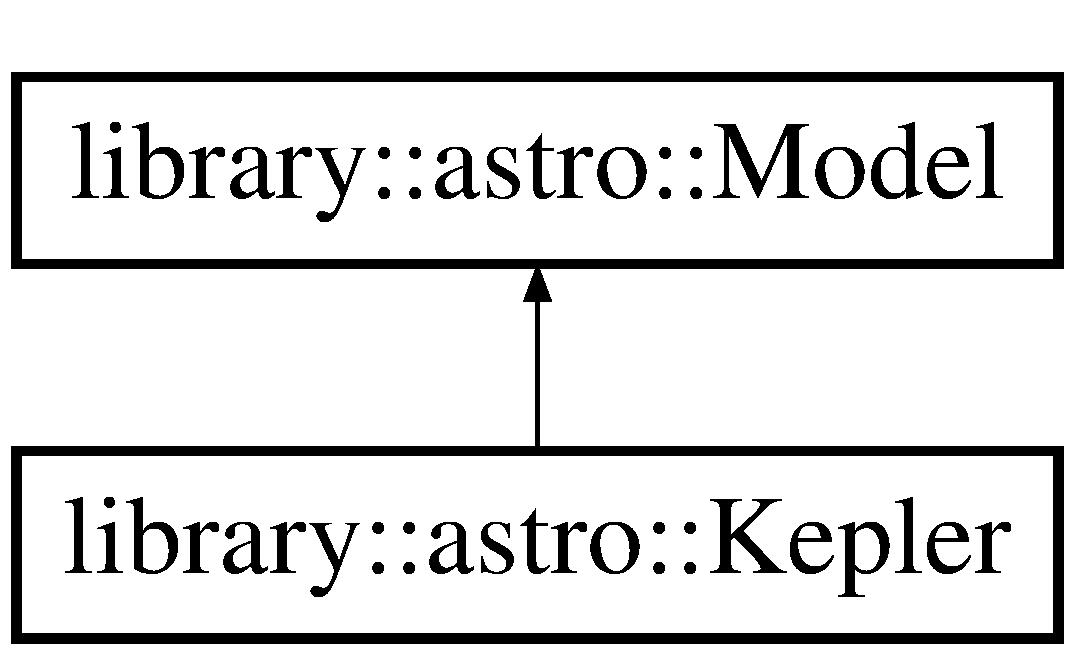
\includegraphics[height=2.000000cm]{classlibrary_1_1astro_1_1_kepler}
\end{center}
\end{figure}
\subsection*{Public Member Functions}
\begin{DoxyCompactItemize}
\item 
\hyperlink{classlibrary_1_1astro_1_1_kepler_a8bba54b94e64c360f5dab3999fde0675}{Kepler} ()
\end{DoxyCompactItemize}


\subsection{Constructor \& Destructor Documentation}
\mbox{\Hypertarget{classlibrary_1_1astro_1_1_kepler_a8bba54b94e64c360f5dab3999fde0675}\label{classlibrary_1_1astro_1_1_kepler_a8bba54b94e64c360f5dab3999fde0675}} 
\index{library\+::astro\+::\+Kepler@{library\+::astro\+::\+Kepler}!Kepler@{Kepler}}
\index{Kepler@{Kepler}!library\+::astro\+::\+Kepler@{library\+::astro\+::\+Kepler}}
\subsubsection{\texorpdfstring{Kepler()}{Kepler()}}
{\footnotesize\ttfamily library\+::astro\+::\+Kepler\+::\+Kepler (\begin{DoxyParamCaption}{ }\end{DoxyParamCaption})}



The documentation for this class was generated from the following file\+:\begin{DoxyCompactItemize}
\item 
include/\+Library/\+Astrodynamics/\+Trajectory/\+Orbit/\+Models/\hyperlink{_kepler_8hpp}{Kepler.\+hpp}\end{DoxyCompactItemize}

\hypertarget{classlibrary_1_1astro_1_1_model}{}\section{library\+:\+:astro\+:\+:Model Class Reference}
\label{classlibrary_1_1astro_1_1_model}\index{library\+::astro\+::\+Model@{library\+::astro\+::\+Model}}


{\ttfamily \#include $<$Model.\+hpp$>$}

Inheritance diagram for library\+:\+:astro\+:\+:Model\+:\begin{figure}[H]
\begin{center}
\leavevmode
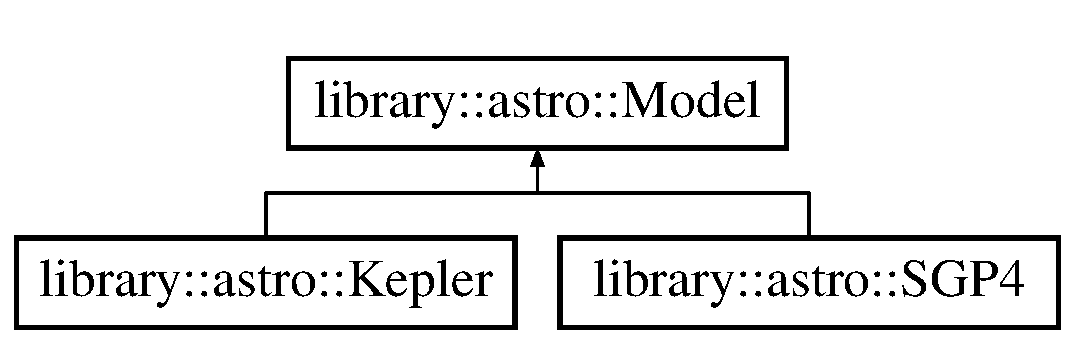
\includegraphics[height=2.000000cm]{classlibrary_1_1astro_1_1_model}
\end{center}
\end{figure}
\subsection*{Public Member Functions}
\begin{DoxyCompactItemize}
\item 
\hyperlink{classlibrary_1_1astro_1_1_model_ad68fa2e75ec873aa8aa2ca136433f59d}{Model} ()
\end{DoxyCompactItemize}


\subsection{Constructor \& Destructor Documentation}
\mbox{\Hypertarget{classlibrary_1_1astro_1_1_model_ad68fa2e75ec873aa8aa2ca136433f59d}\label{classlibrary_1_1astro_1_1_model_ad68fa2e75ec873aa8aa2ca136433f59d}} 
\index{library\+::astro\+::\+Model@{library\+::astro\+::\+Model}!Model@{Model}}
\index{Model@{Model}!library\+::astro\+::\+Model@{library\+::astro\+::\+Model}}
\subsubsection{\texorpdfstring{Model()}{Model()}}
{\footnotesize\ttfamily library\+::astro\+::\+Model\+::\+Model (\begin{DoxyParamCaption}{ }\end{DoxyParamCaption})}



The documentation for this class was generated from the following file\+:\begin{DoxyCompactItemize}
\item 
include/\+Library/\+Astrodynamics/\+Trajectory/\+Orbit/\hyperlink{_model_8hpp}{Model.\+hpp}\end{DoxyCompactItemize}

\hypertarget{classlibrary_1_1astro_1_1_orbit}{}\section{library\+:\+:astro\+:\+:Orbit Class Reference}
\label{classlibrary_1_1astro_1_1_orbit}\index{library\+::astro\+::\+Orbit@{library\+::astro\+::\+Orbit}}


{\ttfamily \#include $<$Orbit.\+hpp$>$}

Inheritance diagram for library\+:\+:astro\+:\+:Orbit\+:\begin{figure}[H]
\begin{center}
\leavevmode
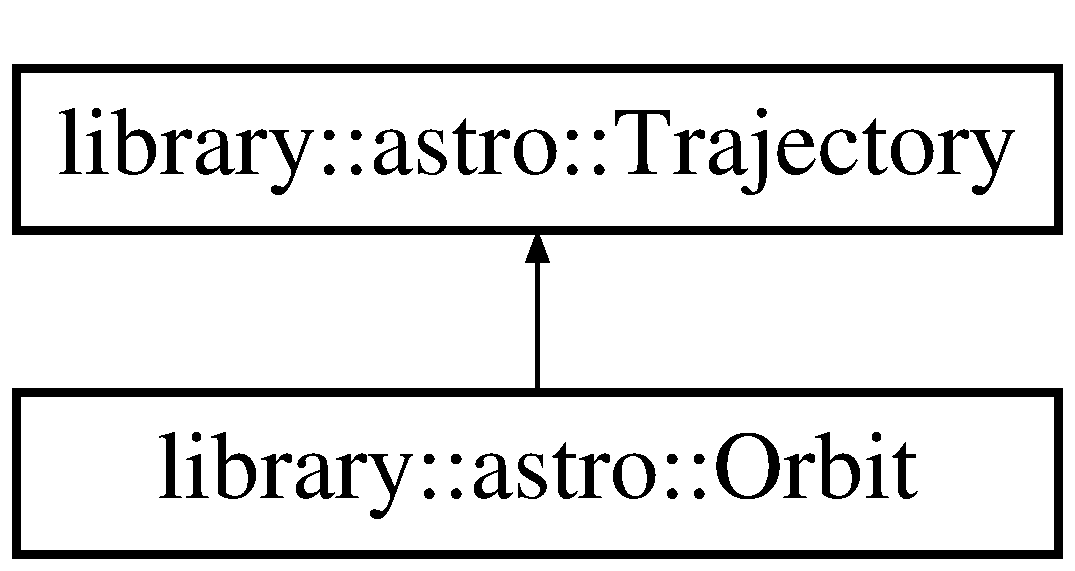
\includegraphics[height=2.000000cm]{classlibrary_1_1astro_1_1_orbit}
\end{center}
\end{figure}
\subsection*{Public Member Functions}
\begin{DoxyCompactItemize}
\item 
\hyperlink{classlibrary_1_1astro_1_1_orbit_a43961ea3c87aab4a726406f36ed193f2}{Orbit} ()
\end{DoxyCompactItemize}


\subsection{Constructor \& Destructor Documentation}
\mbox{\Hypertarget{classlibrary_1_1astro_1_1_orbit_a43961ea3c87aab4a726406f36ed193f2}\label{classlibrary_1_1astro_1_1_orbit_a43961ea3c87aab4a726406f36ed193f2}} 
\index{library\+::astro\+::\+Orbit@{library\+::astro\+::\+Orbit}!Orbit@{Orbit}}
\index{Orbit@{Orbit}!library\+::astro\+::\+Orbit@{library\+::astro\+::\+Orbit}}
\subsubsection{\texorpdfstring{Orbit()}{Orbit()}}
{\footnotesize\ttfamily library\+::astro\+::\+Orbit\+::\+Orbit (\begin{DoxyParamCaption}{ }\end{DoxyParamCaption})}



The documentation for this class was generated from the following file\+:\begin{DoxyCompactItemize}
\item 
include/\+Library/\+Astrodynamics/\+Trajectory/\hyperlink{_orbit_8hpp}{Orbit.\+hpp}\end{DoxyCompactItemize}

\hypertarget{classlibrary_1_1astro_1_1_s_g_p4}{}\section{library\+:\+:astro\+:\+:S\+G\+P4 Class Reference}
\label{classlibrary_1_1astro_1_1_s_g_p4}\index{library\+::astro\+::\+S\+G\+P4@{library\+::astro\+::\+S\+G\+P4}}


{\ttfamily \#include $<$S\+G\+P4.\+hpp$>$}

Inheritance diagram for library\+:\+:astro\+:\+:S\+G\+P4\+:\begin{figure}[H]
\begin{center}
\leavevmode
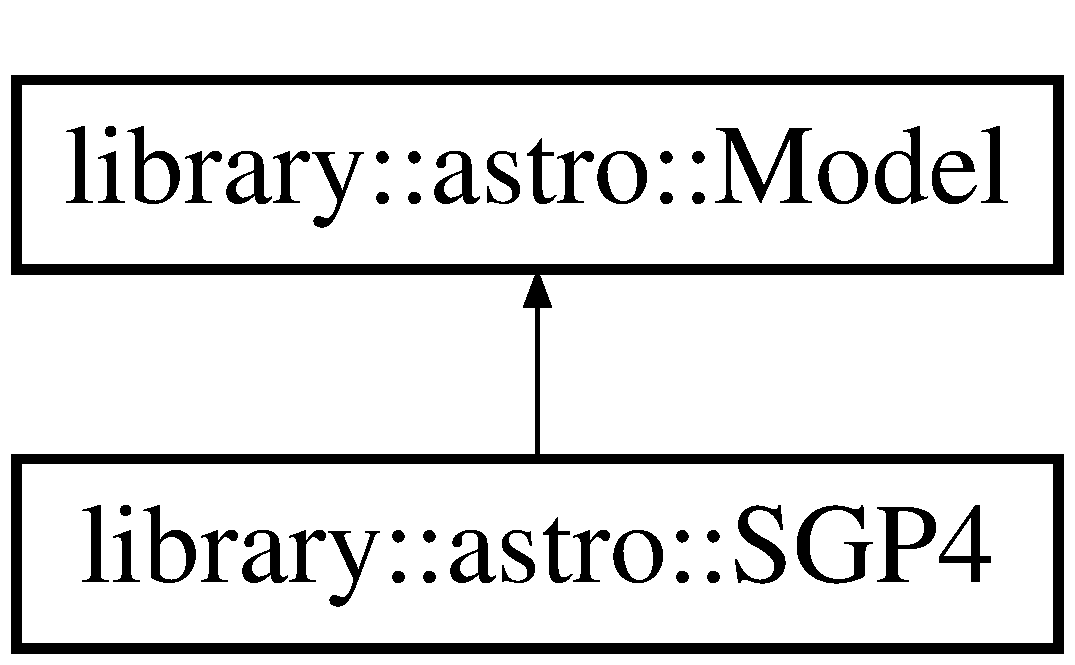
\includegraphics[height=2.000000cm]{classlibrary_1_1astro_1_1_s_g_p4}
\end{center}
\end{figure}
\subsection*{Public Member Functions}
\begin{DoxyCompactItemize}
\item 
\hyperlink{classlibrary_1_1astro_1_1_s_g_p4_a6fb4e1119ce84877ba141a92a3c57b9c}{S\+G\+P4} ()
\end{DoxyCompactItemize}


\subsection{Constructor \& Destructor Documentation}
\mbox{\Hypertarget{classlibrary_1_1astro_1_1_s_g_p4_a6fb4e1119ce84877ba141a92a3c57b9c}\label{classlibrary_1_1astro_1_1_s_g_p4_a6fb4e1119ce84877ba141a92a3c57b9c}} 
\index{library\+::astro\+::\+S\+G\+P4@{library\+::astro\+::\+S\+G\+P4}!S\+G\+P4@{S\+G\+P4}}
\index{S\+G\+P4@{S\+G\+P4}!library\+::astro\+::\+S\+G\+P4@{library\+::astro\+::\+S\+G\+P4}}
\subsubsection{\texorpdfstring{S\+G\+P4()}{SGP4()}}
{\footnotesize\ttfamily library\+::astro\+::\+S\+G\+P4\+::\+S\+G\+P4 (\begin{DoxyParamCaption}{ }\end{DoxyParamCaption})}



The documentation for this class was generated from the following file\+:\begin{DoxyCompactItemize}
\item 
include/\+Library/\+Astrodynamics/\+Trajectory/\+Orbit/\+Models/\hyperlink{_s_g_p4_8hpp}{S\+G\+P4.\+hpp}\end{DoxyCompactItemize}

\hypertarget{classlibrary_1_1astro_1_1_t_l_e}{}\section{library\+:\+:astro\+:\+:T\+LE Class Reference}
\label{classlibrary_1_1astro_1_1_t_l_e}\index{library\+::astro\+::\+T\+LE@{library\+::astro\+::\+T\+LE}}


{\ttfamily \#include $<$T\+L\+E.\+hpp$>$}

\subsection*{Public Member Functions}
\begin{DoxyCompactItemize}
\item 
\hyperlink{classlibrary_1_1astro_1_1_t_l_e_a4ff8b885d24b09f555e8449f6e3f10c0}{T\+LE} ()
\end{DoxyCompactItemize}


\subsection{Constructor \& Destructor Documentation}
\mbox{\Hypertarget{classlibrary_1_1astro_1_1_t_l_e_a4ff8b885d24b09f555e8449f6e3f10c0}\label{classlibrary_1_1astro_1_1_t_l_e_a4ff8b885d24b09f555e8449f6e3f10c0}} 
\index{library\+::astro\+::\+T\+LE@{library\+::astro\+::\+T\+LE}!T\+LE@{T\+LE}}
\index{T\+LE@{T\+LE}!library\+::astro\+::\+T\+LE@{library\+::astro\+::\+T\+LE}}
\subsubsection{\texorpdfstring{T\+L\+E()}{TLE()}}
{\footnotesize\ttfamily library\+::astro\+::\+T\+L\+E\+::\+T\+LE (\begin{DoxyParamCaption}{ }\end{DoxyParamCaption})}



The documentation for this class was generated from the following file\+:\begin{DoxyCompactItemize}
\item 
include/\+Library/\+Astrodynamics/\+Trajectory/\+Orbit/\+Models/\+S\+G\+P4/\hyperlink{_t_l_e_8hpp}{T\+L\+E.\+hpp}\end{DoxyCompactItemize}

\hypertarget{classlibrary_1_1astro_1_1_trajectory}{}\section{library\+:\+:astro\+:\+:Trajectory Class Reference}
\label{classlibrary_1_1astro_1_1_trajectory}\index{library\+::astro\+::\+Trajectory@{library\+::astro\+::\+Trajectory}}


Path followed by an object through space as a function of time.  




{\ttfamily \#include $<$Trajectory.\+hpp$>$}

Inheritance diagram for library\+:\+:astro\+:\+:Trajectory\+:\begin{figure}[H]
\begin{center}
\leavevmode
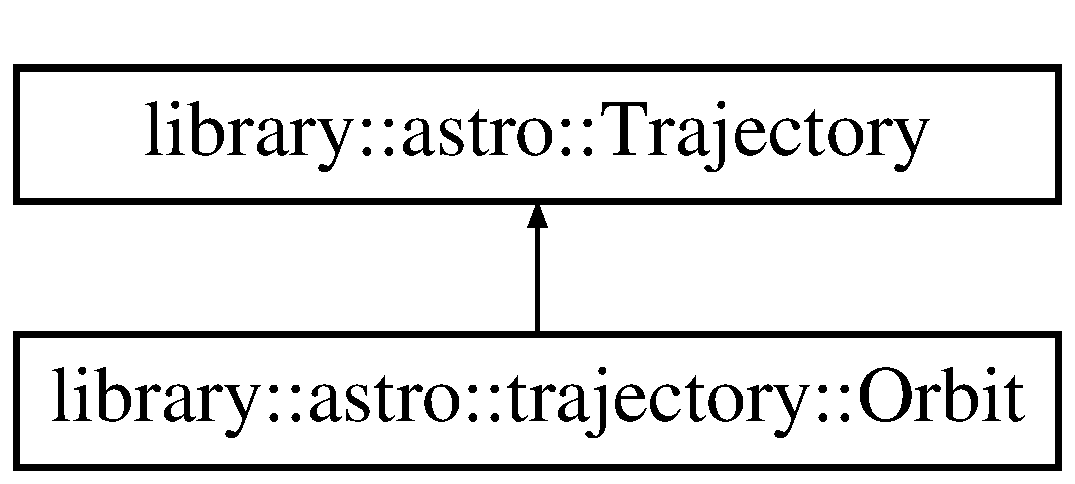
\includegraphics[height=2.000000cm]{classlibrary_1_1astro_1_1_trajectory}
\end{center}
\end{figure}
\subsection*{Public Member Functions}
\begin{DoxyCompactItemize}
\item 
\hyperlink{classlibrary_1_1astro_1_1_trajectory_a8e5c7740915ca947e067c0f419ac1c65}{Trajectory} (const \hyperlink{classlibrary_1_1astro_1_1trajectory_1_1_model}{Model} \&a\+Model)
\begin{DoxyCompactList}\small\item\em Constructor (model) \end{DoxyCompactList}\item 
\hyperlink{classlibrary_1_1astro_1_1_trajectory_abe42247164ca6f966ae5f0c2dfa29182}{Trajectory} (const Array$<$ \hyperlink{classlibrary_1_1astro_1_1trajectory_1_1_state}{State} $>$ \&a\+State\+Array)
\begin{DoxyCompactList}\small\item\em Constructor (state array) \end{DoxyCompactList}\item 
\hyperlink{classlibrary_1_1astro_1_1_trajectory_a63aa2162979ed09fedded192871f0f0a}{Trajectory} (const \hyperlink{classlibrary_1_1astro_1_1_trajectory}{Trajectory} \&a\+Trajectory)
\begin{DoxyCompactList}\small\item\em Copy constructor. \end{DoxyCompactList}\item 
\hyperlink{classlibrary_1_1astro_1_1_trajectory}{Trajectory} \& \hyperlink{classlibrary_1_1astro_1_1_trajectory_abf8200a7b8e08ac9e0f26224fd26cd05}{operator=} (const \hyperlink{classlibrary_1_1astro_1_1_trajectory}{Trajectory} \&a\+Trajectory)=delete
\begin{DoxyCompactList}\small\item\em Copy assignment operator (deleted) \end{DoxyCompactList}\item 
bool \hyperlink{classlibrary_1_1astro_1_1_trajectory_a11bb251602a70c65e727dfc7ed49231e}{operator==} (const \hyperlink{classlibrary_1_1astro_1_1_trajectory}{Trajectory} \&a\+Trajectory) const
\begin{DoxyCompactList}\small\item\em Equal to operator. \end{DoxyCompactList}\item 
bool \hyperlink{classlibrary_1_1astro_1_1_trajectory_a3fa102c5193028fabe84aa7cee9b3e55}{operator!=} (const \hyperlink{classlibrary_1_1astro_1_1_trajectory}{Trajectory} \&a\+Trajectory) const
\begin{DoxyCompactList}\small\item\em Not equal to operator. \end{DoxyCompactList}\item 
bool \hyperlink{classlibrary_1_1astro_1_1_trajectory_aab36edc2566e11d4b5de340cd8230dee}{is\+Defined} () const
\begin{DoxyCompactList}\small\item\em Check if trajectory is defined. \end{DoxyCompactList}\item 
\hyperlink{classlibrary_1_1astro_1_1trajectory_1_1_state}{State} \hyperlink{classlibrary_1_1astro_1_1_trajectory_a5b27c8ad8d547a00ad32c4ab1d63984f}{get\+State\+At} (const Instant \&an\+Instant) const
\begin{DoxyCompactList}\small\item\em Get state at a given instant. \end{DoxyCompactList}\item 
Array$<$ \hyperlink{classlibrary_1_1astro_1_1trajectory_1_1_state}{State} $>$ \hyperlink{classlibrary_1_1astro_1_1_trajectory_a0b7d9ed6012f968b1bfde1f2cc4e34f5}{get\+States\+At} (const Array$<$ Instant $>$ \&an\+Instant\+Array) const
\begin{DoxyCompactList}\small\item\em Get states at a given instants. \end{DoxyCompactList}\item 
virtual void \hyperlink{classlibrary_1_1astro_1_1_trajectory_a6f6afc6bcd8880d7debaa98a79bfa4e6}{print} (std\+::ostream \&an\+Output\+Stream, bool display\+Decorator=true) const
\begin{DoxyCompactList}\small\item\em Print trajectory to output stream. \end{DoxyCompactList}\end{DoxyCompactItemize}
\subsection*{Static Public Member Functions}
\begin{DoxyCompactItemize}
\item 
static \hyperlink{classlibrary_1_1astro_1_1_trajectory}{Trajectory} \hyperlink{classlibrary_1_1astro_1_1_trajectory_a0a8685cabc646fcc5b7f046a606ae967}{Undefined} ()
\begin{DoxyCompactList}\small\item\em Constructs an undefined trajectory. \end{DoxyCompactList}\item 
static \hyperlink{classlibrary_1_1astro_1_1_trajectory}{Trajectory} \hyperlink{classlibrary_1_1astro_1_1_trajectory_a39e9a50f84016cb53ca36d61809dc058}{Position} (const physics\+::coord\+::\+Position \&a\+Position)
\begin{DoxyCompactList}\small\item\em Constructs a trajectory from a given position. \end{DoxyCompactList}\end{DoxyCompactItemize}
\subsection*{Protected Member Functions}
\begin{DoxyCompactItemize}
\item 
const \hyperlink{classlibrary_1_1astro_1_1trajectory_1_1_model}{Model} \& \hyperlink{classlibrary_1_1astro_1_1_trajectory_ac5ebd6f282b52bb3d7c74a79375025e1}{access\+Model} () const
\end{DoxyCompactItemize}
\subsection*{Friends}
\begin{DoxyCompactItemize}
\item 
std\+::ostream \& \hyperlink{classlibrary_1_1astro_1_1_trajectory_aef0327f0240dc2d71eca34dc287f88ea}{operator$<$$<$} (std\+::ostream \&an\+Output\+Stream, const \hyperlink{classlibrary_1_1astro_1_1_trajectory}{Trajectory} \&a\+Trajectory)
\begin{DoxyCompactList}\small\item\em Output stream operator. \end{DoxyCompactList}\end{DoxyCompactItemize}


\subsection{Detailed Description}
Path followed by an object through space as a function of time. 

https\+://en.wikipedia.\+org/wiki/\+Trajectory 

\subsection{Constructor \& Destructor Documentation}
\mbox{\Hypertarget{classlibrary_1_1astro_1_1_trajectory_a8e5c7740915ca947e067c0f419ac1c65}\label{classlibrary_1_1astro_1_1_trajectory_a8e5c7740915ca947e067c0f419ac1c65}} 
\index{library\+::astro\+::\+Trajectory@{library\+::astro\+::\+Trajectory}!Trajectory@{Trajectory}}
\index{Trajectory@{Trajectory}!library\+::astro\+::\+Trajectory@{library\+::astro\+::\+Trajectory}}
\subsubsection{\texorpdfstring{Trajectory()}{Trajectory()}\hspace{0.1cm}{\footnotesize\ttfamily [1/3]}}
{\footnotesize\ttfamily library\+::astro\+::\+Trajectory\+::\+Trajectory (\begin{DoxyParamCaption}\item[{const \hyperlink{classlibrary_1_1astro_1_1trajectory_1_1_model}{Model} \&}]{a\+Model }\end{DoxyParamCaption})}



Constructor (model) 


\begin{DoxyCode}
Tabulated model = \hyperlink{classlibrary_1_1astro_1_1trajectory_1_1models_1_1_tabulated_a63c053c7a308930aa03b354292c85c0f}{Tabulated::Load}(File::Path(Path::Parse(\textcolor{stringliteral}{"/path/to/trajectory.csv"}))) ;
\hyperlink{classlibrary_1_1astro_1_1_trajectory_a8e5c7740915ca947e067c0f419ac1c65}{Trajectory} trajectory = \{ model \} ;
\end{DoxyCode}



\begin{DoxyParams}[1]{Parameters}
\mbox{\tt in}  & {\em a\+Model} & A trajectory model \\
\hline
\end{DoxyParams}
\mbox{\Hypertarget{classlibrary_1_1astro_1_1_trajectory_abe42247164ca6f966ae5f0c2dfa29182}\label{classlibrary_1_1astro_1_1_trajectory_abe42247164ca6f966ae5f0c2dfa29182}} 
\index{library\+::astro\+::\+Trajectory@{library\+::astro\+::\+Trajectory}!Trajectory@{Trajectory}}
\index{Trajectory@{Trajectory}!library\+::astro\+::\+Trajectory@{library\+::astro\+::\+Trajectory}}
\subsubsection{\texorpdfstring{Trajectory()}{Trajectory()}\hspace{0.1cm}{\footnotesize\ttfamily [2/3]}}
{\footnotesize\ttfamily library\+::astro\+::\+Trajectory\+::\+Trajectory (\begin{DoxyParamCaption}\item[{const Array$<$ \hyperlink{classlibrary_1_1astro_1_1trajectory_1_1_state}{State} $>$ \&}]{a\+State\+Array }\end{DoxyParamCaption})}



Constructor (state array) 


\begin{DoxyCode}
Array<State> stateArray = \{ ... \} ;
\hyperlink{classlibrary_1_1astro_1_1_trajectory_a8e5c7740915ca947e067c0f419ac1c65}{Trajectory} trajectory = \{ stateArray \} ;
\end{DoxyCode}



\begin{DoxyParams}[1]{Parameters}
\mbox{\tt in}  & {\em a\+State\+Array} & An array of states \\
\hline
\end{DoxyParams}
\mbox{\Hypertarget{classlibrary_1_1astro_1_1_trajectory_a63aa2162979ed09fedded192871f0f0a}\label{classlibrary_1_1astro_1_1_trajectory_a63aa2162979ed09fedded192871f0f0a}} 
\index{library\+::astro\+::\+Trajectory@{library\+::astro\+::\+Trajectory}!Trajectory@{Trajectory}}
\index{Trajectory@{Trajectory}!library\+::astro\+::\+Trajectory@{library\+::astro\+::\+Trajectory}}
\subsubsection{\texorpdfstring{Trajectory()}{Trajectory()}\hspace{0.1cm}{\footnotesize\ttfamily [3/3]}}
{\footnotesize\ttfamily library\+::astro\+::\+Trajectory\+::\+Trajectory (\begin{DoxyParamCaption}\item[{const \hyperlink{classlibrary_1_1astro_1_1_trajectory}{Trajectory} \&}]{a\+Trajectory }\end{DoxyParamCaption})}



Copy constructor. 


\begin{DoxyParams}[1]{Parameters}
\mbox{\tt in}  & {\em a\+Trajectory} & A trajectory \\
\hline
\end{DoxyParams}


\subsection{Member Function Documentation}
\mbox{\Hypertarget{classlibrary_1_1astro_1_1_trajectory_ac5ebd6f282b52bb3d7c74a79375025e1}\label{classlibrary_1_1astro_1_1_trajectory_ac5ebd6f282b52bb3d7c74a79375025e1}} 
\index{library\+::astro\+::\+Trajectory@{library\+::astro\+::\+Trajectory}!access\+Model@{access\+Model}}
\index{access\+Model@{access\+Model}!library\+::astro\+::\+Trajectory@{library\+::astro\+::\+Trajectory}}
\subsubsection{\texorpdfstring{access\+Model()}{accessModel()}}
{\footnotesize\ttfamily const \hyperlink{classlibrary_1_1astro_1_1trajectory_1_1_model}{Model} \& library\+::astro\+::\+Trajectory\+::access\+Model (\begin{DoxyParamCaption}{ }\end{DoxyParamCaption}) const\hspace{0.3cm}{\ttfamily [protected]}}

\mbox{\Hypertarget{classlibrary_1_1astro_1_1_trajectory_a5b27c8ad8d547a00ad32c4ab1d63984f}\label{classlibrary_1_1astro_1_1_trajectory_a5b27c8ad8d547a00ad32c4ab1d63984f}} 
\index{library\+::astro\+::\+Trajectory@{library\+::astro\+::\+Trajectory}!get\+State\+At@{get\+State\+At}}
\index{get\+State\+At@{get\+State\+At}!library\+::astro\+::\+Trajectory@{library\+::astro\+::\+Trajectory}}
\subsubsection{\texorpdfstring{get\+State\+At()}{getStateAt()}}
{\footnotesize\ttfamily \hyperlink{classlibrary_1_1astro_1_1trajectory_1_1_state}{State} library\+::astro\+::\+Trajectory\+::get\+State\+At (\begin{DoxyParamCaption}\item[{const Instant \&}]{an\+Instant }\end{DoxyParamCaption}) const}



Get state at a given instant. 


\begin{DoxyCode}
\hyperlink{classlibrary_1_1astro_1_1_trajectory_a8e5c7740915ca947e067c0f419ac1c65}{Trajectory} trajectory = \{ ... \} ;
Instant instant = \{ ... \} ;
State state = trajectory.getStateAt(instant) ;
\end{DoxyCode}



\begin{DoxyParams}[1]{Parameters}
\mbox{\tt in}  & {\em an\+Instant} & An instant \\
\hline
\end{DoxyParams}
\begin{DoxyReturn}{Returns}
State 
\end{DoxyReturn}
\mbox{\Hypertarget{classlibrary_1_1astro_1_1_trajectory_a0b7d9ed6012f968b1bfde1f2cc4e34f5}\label{classlibrary_1_1astro_1_1_trajectory_a0b7d9ed6012f968b1bfde1f2cc4e34f5}} 
\index{library\+::astro\+::\+Trajectory@{library\+::astro\+::\+Trajectory}!get\+States\+At@{get\+States\+At}}
\index{get\+States\+At@{get\+States\+At}!library\+::astro\+::\+Trajectory@{library\+::astro\+::\+Trajectory}}
\subsubsection{\texorpdfstring{get\+States\+At()}{getStatesAt()}}
{\footnotesize\ttfamily Array$<$ \hyperlink{classlibrary_1_1astro_1_1trajectory_1_1_state}{State} $>$ library\+::astro\+::\+Trajectory\+::get\+States\+At (\begin{DoxyParamCaption}\item[{const Array$<$ Instant $>$ \&}]{an\+Instant\+Array }\end{DoxyParamCaption}) const}



Get states at a given instants. 


\begin{DoxyCode}
\hyperlink{classlibrary_1_1astro_1_1_trajectory_a8e5c7740915ca947e067c0f419ac1c65}{Trajectory} trajectory = \{ ... \} ;
Array<Instant> instants = \{ ... \} ;
Array<State> state = trajectory.getStatesAt(instants) ;
\end{DoxyCode}



\begin{DoxyParams}[1]{Parameters}
\mbox{\tt in}  & {\em an\+Instant\+Array} & An array of instants \\
\hline
\end{DoxyParams}
\begin{DoxyReturn}{Returns}
Array of states 
\end{DoxyReturn}
\mbox{\Hypertarget{classlibrary_1_1astro_1_1_trajectory_aab36edc2566e11d4b5de340cd8230dee}\label{classlibrary_1_1astro_1_1_trajectory_aab36edc2566e11d4b5de340cd8230dee}} 
\index{library\+::astro\+::\+Trajectory@{library\+::astro\+::\+Trajectory}!is\+Defined@{is\+Defined}}
\index{is\+Defined@{is\+Defined}!library\+::astro\+::\+Trajectory@{library\+::astro\+::\+Trajectory}}
\subsubsection{\texorpdfstring{is\+Defined()}{isDefined()}}
{\footnotesize\ttfamily bool library\+::astro\+::\+Trajectory\+::is\+Defined (\begin{DoxyParamCaption}{ }\end{DoxyParamCaption}) const}



Check if trajectory is defined. 


\begin{DoxyCode}
\hyperlink{classlibrary_1_1astro_1_1_trajectory_a8e5c7740915ca947e067c0f419ac1c65}{Trajectory}(...).isDefined() ;
\end{DoxyCode}


\begin{DoxyReturn}{Returns}
True if trajectory is defined 
\end{DoxyReturn}
\mbox{\Hypertarget{classlibrary_1_1astro_1_1_trajectory_a3fa102c5193028fabe84aa7cee9b3e55}\label{classlibrary_1_1astro_1_1_trajectory_a3fa102c5193028fabe84aa7cee9b3e55}} 
\index{library\+::astro\+::\+Trajectory@{library\+::astro\+::\+Trajectory}!operator"!=@{operator"!=}}
\index{operator"!=@{operator"!=}!library\+::astro\+::\+Trajectory@{library\+::astro\+::\+Trajectory}}
\subsubsection{\texorpdfstring{operator"!=()}{operator!=()}}
{\footnotesize\ttfamily bool library\+::astro\+::\+Trajectory\+::operator!= (\begin{DoxyParamCaption}\item[{const \hyperlink{classlibrary_1_1astro_1_1_trajectory}{Trajectory} \&}]{a\+Trajectory }\end{DoxyParamCaption}) const}



Not equal to operator. 


\begin{DoxyCode}
\hyperlink{classlibrary_1_1astro_1_1_trajectory_a8e5c7740915ca947e067c0f419ac1c65}{Trajectory}(...) != \hyperlink{classlibrary_1_1astro_1_1_trajectory_a8e5c7740915ca947e067c0f419ac1c65}{Trajectory}(...) ;
\end{DoxyCode}



\begin{DoxyParams}[1]{Parameters}
\mbox{\tt in}  & {\em a\+Trajectory} & A trajectory \\
\hline
\end{DoxyParams}
\begin{DoxyReturn}{Returns}
True if trajectories are not equal 
\end{DoxyReturn}
\mbox{\Hypertarget{classlibrary_1_1astro_1_1_trajectory_abf8200a7b8e08ac9e0f26224fd26cd05}\label{classlibrary_1_1astro_1_1_trajectory_abf8200a7b8e08ac9e0f26224fd26cd05}} 
\index{library\+::astro\+::\+Trajectory@{library\+::astro\+::\+Trajectory}!operator=@{operator=}}
\index{operator=@{operator=}!library\+::astro\+::\+Trajectory@{library\+::astro\+::\+Trajectory}}
\subsubsection{\texorpdfstring{operator=()}{operator=()}}
{\footnotesize\ttfamily \hyperlink{classlibrary_1_1astro_1_1_trajectory}{Trajectory}\& library\+::astro\+::\+Trajectory\+::operator= (\begin{DoxyParamCaption}\item[{const \hyperlink{classlibrary_1_1astro_1_1_trajectory}{Trajectory} \&}]{a\+Trajectory }\end{DoxyParamCaption})\hspace{0.3cm}{\ttfamily [delete]}}



Copy assignment operator (deleted) 

\mbox{\Hypertarget{classlibrary_1_1astro_1_1_trajectory_a11bb251602a70c65e727dfc7ed49231e}\label{classlibrary_1_1astro_1_1_trajectory_a11bb251602a70c65e727dfc7ed49231e}} 
\index{library\+::astro\+::\+Trajectory@{library\+::astro\+::\+Trajectory}!operator==@{operator==}}
\index{operator==@{operator==}!library\+::astro\+::\+Trajectory@{library\+::astro\+::\+Trajectory}}
\subsubsection{\texorpdfstring{operator==()}{operator==()}}
{\footnotesize\ttfamily bool library\+::astro\+::\+Trajectory\+::operator== (\begin{DoxyParamCaption}\item[{const \hyperlink{classlibrary_1_1astro_1_1_trajectory}{Trajectory} \&}]{a\+Trajectory }\end{DoxyParamCaption}) const}



Equal to operator. 


\begin{DoxyCode}
\hyperlink{classlibrary_1_1astro_1_1_trajectory_a8e5c7740915ca947e067c0f419ac1c65}{Trajectory}(...) == \hyperlink{classlibrary_1_1astro_1_1_trajectory_a8e5c7740915ca947e067c0f419ac1c65}{Trajectory}(...) ;
\end{DoxyCode}



\begin{DoxyParams}[1]{Parameters}
\mbox{\tt in}  & {\em a\+Trajectory} & A trajectory \\
\hline
\end{DoxyParams}
\begin{DoxyReturn}{Returns}
True if trajectories are equal 
\end{DoxyReturn}
\mbox{\Hypertarget{classlibrary_1_1astro_1_1_trajectory_a39e9a50f84016cb53ca36d61809dc058}\label{classlibrary_1_1astro_1_1_trajectory_a39e9a50f84016cb53ca36d61809dc058}} 
\index{library\+::astro\+::\+Trajectory@{library\+::astro\+::\+Trajectory}!Position@{Position}}
\index{Position@{Position}!library\+::astro\+::\+Trajectory@{library\+::astro\+::\+Trajectory}}
\subsubsection{\texorpdfstring{Position()}{Position()}}
{\footnotesize\ttfamily \hyperlink{classlibrary_1_1astro_1_1_trajectory}{Trajectory} library\+::astro\+::\+Trajectory\+::\+Position (\begin{DoxyParamCaption}\item[{const physics\+::coord\+::\+Position \&}]{a\+Position }\end{DoxyParamCaption})\hspace{0.3cm}{\ttfamily [static]}}



Constructs a trajectory from a given position. 


\begin{DoxyCode}
\hyperlink{classlibrary_1_1astro_1_1_trajectory_a39e9a50f84016cb53ca36d61809dc058}{Position} position = Position::Meters(\{ 0.0, 0.0, 0.0 \}, Frame::GCRF()) ;
\hyperlink{classlibrary_1_1astro_1_1_trajectory_a8e5c7740915ca947e067c0f419ac1c65}{Trajectory} trajectory = \hyperlink{classlibrary_1_1astro_1_1_trajectory_a39e9a50f84016cb53ca36d61809dc058}{Trajectory::Position}(position) ;
\end{DoxyCode}


\begin{DoxyReturn}{Returns}
Static trajectory 
\end{DoxyReturn}
\mbox{\Hypertarget{classlibrary_1_1astro_1_1_trajectory_a6f6afc6bcd8880d7debaa98a79bfa4e6}\label{classlibrary_1_1astro_1_1_trajectory_a6f6afc6bcd8880d7debaa98a79bfa4e6}} 
\index{library\+::astro\+::\+Trajectory@{library\+::astro\+::\+Trajectory}!print@{print}}
\index{print@{print}!library\+::astro\+::\+Trajectory@{library\+::astro\+::\+Trajectory}}
\subsubsection{\texorpdfstring{print()}{print()}}
{\footnotesize\ttfamily void library\+::astro\+::\+Trajectory\+::print (\begin{DoxyParamCaption}\item[{std\+::ostream \&}]{an\+Output\+Stream,  }\item[{bool}]{display\+Decorator = {\ttfamily true} }\end{DoxyParamCaption}) const\hspace{0.3cm}{\ttfamily [virtual]}}



Print trajectory to output stream. 


\begin{DoxyCode}
\hyperlink{classlibrary_1_1astro_1_1_trajectory_a8e5c7740915ca947e067c0f419ac1c65}{Trajectory} trajectory = \{ ... \} ;
trajectory.print(std::cout, \textcolor{keyword}{true}) ;
\end{DoxyCode}



\begin{DoxyParams}[1]{Parameters}
\mbox{\tt in}  & {\em an\+Output\+Stream} & An output stream \\
\hline
\mbox{\tt in}  & {\em display\+Decorator} & If true, display decorator \\
\hline
\end{DoxyParams}


Reimplemented in \hyperlink{classlibrary_1_1astro_1_1trajectory_1_1_orbit_ac3b8c212e5b66822ab7eb09785a6c228}{library\+::astro\+::trajectory\+::\+Orbit}.

\mbox{\Hypertarget{classlibrary_1_1astro_1_1_trajectory_a0a8685cabc646fcc5b7f046a606ae967}\label{classlibrary_1_1astro_1_1_trajectory_a0a8685cabc646fcc5b7f046a606ae967}} 
\index{library\+::astro\+::\+Trajectory@{library\+::astro\+::\+Trajectory}!Undefined@{Undefined}}
\index{Undefined@{Undefined}!library\+::astro\+::\+Trajectory@{library\+::astro\+::\+Trajectory}}
\subsubsection{\texorpdfstring{Undefined()}{Undefined()}}
{\footnotesize\ttfamily \hyperlink{classlibrary_1_1astro_1_1_trajectory}{Trajectory} library\+::astro\+::\+Trajectory\+::\+Undefined (\begin{DoxyParamCaption}{ }\end{DoxyParamCaption})\hspace{0.3cm}{\ttfamily [static]}}



Constructs an undefined trajectory. 


\begin{DoxyCode}
\hyperlink{classlibrary_1_1astro_1_1_trajectory_a8e5c7740915ca947e067c0f419ac1c65}{Trajectory} trajectory = \hyperlink{classlibrary_1_1astro_1_1_trajectory_a0a8685cabc646fcc5b7f046a606ae967}{Trajectory::Undefined}() ; \textcolor{comment}{// Undefined}
\end{DoxyCode}


\begin{DoxyReturn}{Returns}
Undefined trajectory 
\end{DoxyReturn}


\subsection{Friends And Related Function Documentation}
\mbox{\Hypertarget{classlibrary_1_1astro_1_1_trajectory_aef0327f0240dc2d71eca34dc287f88ea}\label{classlibrary_1_1astro_1_1_trajectory_aef0327f0240dc2d71eca34dc287f88ea}} 
\index{library\+::astro\+::\+Trajectory@{library\+::astro\+::\+Trajectory}!operator$<$$<$@{operator$<$$<$}}
\index{operator$<$$<$@{operator$<$$<$}!library\+::astro\+::\+Trajectory@{library\+::astro\+::\+Trajectory}}
\subsubsection{\texorpdfstring{operator$<$$<$}{operator<<}}
{\footnotesize\ttfamily std\+::ostream\& operator$<$$<$ (\begin{DoxyParamCaption}\item[{std\+::ostream \&}]{an\+Output\+Stream,  }\item[{const \hyperlink{classlibrary_1_1astro_1_1_trajectory}{Trajectory} \&}]{a\+Trajectory }\end{DoxyParamCaption})\hspace{0.3cm}{\ttfamily [friend]}}



Output stream operator. 


\begin{DoxyCode}
std::cout << \hyperlink{classlibrary_1_1astro_1_1_trajectory_a8e5c7740915ca947e067c0f419ac1c65}{Trajectory}(...) ;
\end{DoxyCode}



\begin{DoxyParams}[1]{Parameters}
\mbox{\tt in}  & {\em an\+Output\+Stream} & An output stream \\
\hline
\mbox{\tt in}  & {\em a\+Trajectory} & A trajectory \\
\hline
\end{DoxyParams}
\begin{DoxyReturn}{Returns}
A reference to output stream 
\end{DoxyReturn}


The documentation for this class was generated from the following files\+:\begin{DoxyCompactItemize}
\item 
include/\+Library/\+Astrodynamics/\hyperlink{_trajectory_8hpp}{Trajectory.\+hpp}\item 
src/\+Library/\+Astrodynamics/\hyperlink{_trajectory_8cpp}{Trajectory.\+cpp}\end{DoxyCompactItemize}

\chapter{File Documentation}
\hypertarget{_c_o_n_t_r_i_b_u_t_i_n_g_8md}{}\section{C\+O\+N\+T\+R\+I\+B\+U\+T\+I\+N\+G.\+md File Reference}
\label{_c_o_n_t_r_i_b_u_t_i_n_g_8md}\index{C\+O\+N\+T\+R\+I\+B\+U\+T\+I\+N\+G.\+md@{C\+O\+N\+T\+R\+I\+B\+U\+T\+I\+N\+G.\+md}}

\hypertarget{_tutorial_8md}{}\section{docs/\+Tutorial.md File Reference}
\label{_tutorial_8md}\index{docs/\+Tutorial.\+md@{docs/\+Tutorial.\+md}}

\hypertarget{_access_8hpp}{}\section{include/\+Open\+Space\+Toolkit/\+Astrodynamics/\+Access.hpp File Reference}
\label{_access_8hpp}\index{include/\+Open\+Space\+Toolkit/\+Astrodynamics/\+Access.\+hpp@{include/\+Open\+Space\+Toolkit/\+Astrodynamics/\+Access.\+hpp}}
{\ttfamily \#include $<$Open\+Space\+Toolkit/\+Physics/\+Time/\+Interval.\+hpp$>$}\newline
{\ttfamily \#include $<$Open\+Space\+Toolkit/\+Physics/\+Time/\+Duration.\+hpp$>$}\newline
{\ttfamily \#include $<$Open\+Space\+Toolkit/\+Physics/\+Time/\+Instant.\+hpp$>$}\newline
{\ttfamily \#include $<$Open\+Space\+Toolkit/\+Core/\+Containers/\+Array.\+hpp$>$}\newline
{\ttfamily \#include $<$Open\+Space\+Toolkit/\+Core/\+Types/\+String.\+hpp$>$}\newline
\subsection*{Classes}
\begin{DoxyCompactItemize}
\item 
class \hyperlink{classostk_1_1astro_1_1_access}{ostk\+::astro\+::\+Access}
\begin{DoxyCompactList}\small\item\em Object-\/to-\/object visibility. \end{DoxyCompactList}\end{DoxyCompactItemize}
\subsection*{Namespaces}
\begin{DoxyCompactItemize}
\item 
 \hyperlink{namespaceostk}{ostk}
\item 
 \hyperlink{namespaceostk_1_1astro}{ostk\+::astro}
\end{DoxyCompactItemize}


\subsection{Detailed Description}
Open Space Toolkit ▸ Astrodynamics

\begin{DoxyAuthor}{Author}
Lucas Brémond \href{mailto:lucas@loftorbital.com}{\tt lucas@loftorbital.\+com}  Apache License 2.\+0 
\end{DoxyAuthor}

\hypertarget{_trajectory_8hpp}{}\section{include/\+Library/\+Astrodynamics/\+Trajectory.hpp File Reference}
\label{_trajectory_8hpp}\index{include/\+Library/\+Astrodynamics/\+Trajectory.\+hpp@{include/\+Library/\+Astrodynamics/\+Trajectory.\+hpp}}
{\ttfamily \#include $<$Library/\+Astrodynamics/\+Trajectory/\+State.\+hpp$>$}\newline
{\ttfamily \#include $<$Library/\+Astrodynamics/\+Trajectory/\+Model.\+hpp$>$}\newline
{\ttfamily \#include $<$Library/\+Physics/\+Coordinate/\+Position.\+hpp$>$}\newline
{\ttfamily \#include $<$Library/\+Physics/\+Time/\+Interval.\+hpp$>$}\newline
{\ttfamily \#include $<$Library/\+Physics/\+Time/\+Instant.\+hpp$>$}\newline
{\ttfamily \#include $<$Library/\+Core/\+Containers/\+Array.\+hpp$>$}\newline
{\ttfamily \#include $<$Library/\+Core/\+Types/\+String.\+hpp$>$}\newline
{\ttfamily \#include $<$Library/\+Core/\+Types/\+Index.\+hpp$>$}\newline
{\ttfamily \#include $<$Library/\+Core/\+Types/\+Unique.\+hpp$>$}\newline
\subsection*{Classes}
\begin{DoxyCompactItemize}
\item 
class \hyperlink{classlibrary_1_1astro_1_1_trajectory}{library\+::astro\+::\+Trajectory}
\begin{DoxyCompactList}\small\item\em Path followed by an object through space as a function of time. \end{DoxyCompactList}\end{DoxyCompactItemize}
\subsection*{Namespaces}
\begin{DoxyCompactItemize}
\item 
 \hyperlink{namespacelibrary}{library}
\item 
 \hyperlink{namespacelibrary_1_1astro}{library\+::astro}
\end{DoxyCompactItemize}


\subsection{Detailed Description}
Library/\+Astrodynamics

\begin{DoxyAuthor}{Author}
Lucas Brémond \href{mailto:lucas@loftorbital.com}{\tt lucas@loftorbital.\+com}  T\+BD 
\end{DoxyAuthor}

\hypertarget{_orbit_8hpp}{}\section{include/\+Open\+Space\+Toolkit/\+Astrodynamics/\+Trajectory/\+Orbit.hpp File Reference}
\label{_orbit_8hpp}\index{include/\+Open\+Space\+Toolkit/\+Astrodynamics/\+Trajectory/\+Orbit.\+hpp@{include/\+Open\+Space\+Toolkit/\+Astrodynamics/\+Trajectory/\+Orbit.\+hpp}}
{\ttfamily \#include $<$Open\+Space\+Toolkit/\+Astrodynamics/\+Trajectory/\+Orbit/\+Model.\+hpp$>$}\newline
{\ttfamily \#include $<$Open\+Space\+Toolkit/\+Astrodynamics/\+Trajectory/\+Orbit/\+Pass.\+hpp$>$}\newline
{\ttfamily \#include $<$Open\+Space\+Toolkit/\+Astrodynamics/\+Trajectory/\+State.\+hpp$>$}\newline
{\ttfamily \#include $<$Open\+Space\+Toolkit/\+Astrodynamics/\+Trajectory.\+hpp$>$}\newline
{\ttfamily \#include $<$Open\+Space\+Toolkit/\+Physics/\+Environment/\+Objects/\+Celestial.\+hpp$>$}\newline
{\ttfamily \#include $<$Open\+Space\+Toolkit/\+Physics/\+Coordinate/\+Frame.\+hpp$>$}\newline
{\ttfamily \#include $<$Open\+Space\+Toolkit/\+Physics/\+Time/\+Time.\+hpp$>$}\newline
{\ttfamily \#include $<$Open\+Space\+Toolkit/\+Physics/\+Time/\+Instant.\+hpp$>$}\newline
{\ttfamily \#include $<$Open\+Space\+Toolkit/\+Physics/\+Units/\+Derived/\+Angle.\+hpp$>$}\newline
{\ttfamily \#include $<$Open\+Space\+Toolkit/\+Physics/\+Units/\+Length.\+hpp$>$}\newline
{\ttfamily \#include $<$Open\+Space\+Toolkit/\+Core/\+Containers/\+Map.\+hpp$>$}\newline
{\ttfamily \#include $<$Open\+Space\+Toolkit/\+Core/\+Containers/\+Array.\+hpp$>$}\newline
{\ttfamily \#include $<$Open\+Space\+Toolkit/\+Core/\+Types/\+Real.\+hpp$>$}\newline
{\ttfamily \#include $<$Open\+Space\+Toolkit/\+Core/\+Types/\+Integer.\+hpp$>$}\newline
{\ttfamily \#include $<$Open\+Space\+Toolkit/\+Core/\+Types/\+Index.\+hpp$>$}\newline
{\ttfamily \#include $<$Open\+Space\+Toolkit/\+Core/\+Types/\+Shared.\+hpp$>$}\newline
{\ttfamily \#include $<$Open\+Space\+Toolkit/\+Core/\+Types/\+Unique.\+hpp$>$}\newline
{\ttfamily \#include $<$mutex$>$}\newline
\subsection*{Classes}
\begin{DoxyCompactItemize}
\item 
class \hyperlink{classostk_1_1astro_1_1trajectory_1_1_orbit}{ostk\+::astro\+::trajectory\+::\+Orbit}
\begin{DoxyCompactList}\small\item\em Gravitationally curved trajectory of an object. \end{DoxyCompactList}\end{DoxyCompactItemize}
\subsection*{Namespaces}
\begin{DoxyCompactItemize}
\item 
 \hyperlink{namespaceostk}{ostk}
\item 
 \hyperlink{namespaceostk_1_1astro}{ostk\+::astro}
\item 
 \hyperlink{namespaceostk_1_1astro_1_1trajectory}{ostk\+::astro\+::trajectory}
\end{DoxyCompactItemize}


\subsection{Detailed Description}
Open Space Toolkit ▸ Astrodynamics

\begin{DoxyAuthor}{Author}
Lucas Brémond \href{mailto:lucas@loftorbital.com}{\tt lucas@loftorbital.\+com}  Apache License 2.\+0 
\end{DoxyAuthor}

\hypertarget{_model_8hpp}{}\section{include/\+Library/\+Astrodynamics/\+Trajectory/\+Orbit/\+Model.hpp File Reference}
\label{_model_8hpp}\index{include/\+Library/\+Astrodynamics/\+Trajectory/\+Orbit/\+Model.\+hpp@{include/\+Library/\+Astrodynamics/\+Trajectory/\+Orbit/\+Model.\+hpp}}
{\ttfamily \#include $<$Library/\+Core/\+Types/\+String.\+hpp$>$}\newline
{\ttfamily \#include $<$Library/\+Core/\+Types/\+Real.\+hpp$>$}\newline
\subsection*{Classes}
\begin{DoxyCompactItemize}
\item 
class \hyperlink{classlibrary_1_1astro_1_1_model}{library\+::astro\+::\+Model}
\end{DoxyCompactItemize}
\subsection*{Namespaces}
\begin{DoxyCompactItemize}
\item 
 \hyperlink{namespacelibrary}{library}
\item 
 \hyperlink{namespacelibrary_1_1astro}{library\+::astro}
\end{DoxyCompactItemize}


\subsection{Detailed Description}
Library/\+Astrodynamics

\begin{DoxyAuthor}{Author}
Lucas Brémond \href{mailto:lucas@loftorbital.com}{\tt lucas@loftorbital.\+com}  T\+BD 
\end{DoxyAuthor}

\hypertarget{_kepler_8hpp}{}\section{include/\+Library/\+Astrodynamics/\+Trajectory/\+Orbit/\+Models/\+Kepler.hpp File Reference}
\label{_kepler_8hpp}\index{include/\+Library/\+Astrodynamics/\+Trajectory/\+Orbit/\+Models/\+Kepler.\+hpp@{include/\+Library/\+Astrodynamics/\+Trajectory/\+Orbit/\+Models/\+Kepler.\+hpp}}
{\ttfamily \#include $<$Library/\+Astrodynamics/\+Trajectory/\+Orbit/\+Model.\+hpp$>$}\newline
{\ttfamily \#include $<$Library/\+Core/\+Types/\+String.\+hpp$>$}\newline
{\ttfamily \#include $<$Library/\+Core/\+Types/\+Real.\+hpp$>$}\newline
\subsection*{Classes}
\begin{DoxyCompactItemize}
\item 
class \hyperlink{classlibrary_1_1astro_1_1_kepler}{library\+::astro\+::\+Kepler}
\end{DoxyCompactItemize}
\subsection*{Namespaces}
\begin{DoxyCompactItemize}
\item 
 \hyperlink{namespacelibrary}{library}
\item 
 \hyperlink{namespacelibrary_1_1astro}{library\+::astro}
\end{DoxyCompactItemize}


\subsection{Detailed Description}
Library/\+Astrodynamics

\begin{DoxyAuthor}{Author}
Lucas Brémond \href{mailto:lucas@loftorbital.com}{\tt lucas@loftorbital.\+com}  T\+BD 
\end{DoxyAuthor}

\hypertarget{_c_o_e_8hpp}{}\section{include/\+Open\+Space\+Toolkit/\+Astrodynamics/\+Trajectory/\+Orbit/\+Models/\+Kepler/\+C\+OE.hpp File Reference}
\label{_c_o_e_8hpp}\index{include/\+Open\+Space\+Toolkit/\+Astrodynamics/\+Trajectory/\+Orbit/\+Models/\+Kepler/\+C\+O\+E.\+hpp@{include/\+Open\+Space\+Toolkit/\+Astrodynamics/\+Trajectory/\+Orbit/\+Models/\+Kepler/\+C\+O\+E.\+hpp}}
{\ttfamily \#include $<$Open\+Space\+Toolkit/\+Physics/\+Coordinate/\+Frame.\+hpp$>$}\newline
{\ttfamily \#include $<$Open\+Space\+Toolkit/\+Physics/\+Coordinate/\+Velocity.\+hpp$>$}\newline
{\ttfamily \#include $<$Open\+Space\+Toolkit/\+Physics/\+Coordinate/\+Position.\+hpp$>$}\newline
{\ttfamily \#include $<$Open\+Space\+Toolkit/\+Physics/\+Time/\+Duration.\+hpp$>$}\newline
{\ttfamily \#include $<$Open\+Space\+Toolkit/\+Physics/\+Units/\+Derived/\+Angle.\+hpp$>$}\newline
{\ttfamily \#include $<$Open\+Space\+Toolkit/\+Physics/\+Units/\+Derived.\+hpp$>$}\newline
{\ttfamily \#include $<$Open\+Space\+Toolkit/\+Physics/\+Units/\+Length.\+hpp$>$}\newline
{\ttfamily \#include $<$Open\+Space\+Toolkit/\+Core/\+Containers/\+Pair.\+hpp$>$}\newline
{\ttfamily \#include $<$Open\+Space\+Toolkit/\+Core/\+Types/\+Real.\+hpp$>$}\newline
{\ttfamily \#include $<$Open\+Space\+Toolkit/\+Core/\+Types/\+Shared.\+hpp$>$}\newline
\subsection*{Classes}
\begin{DoxyCompactItemize}
\item 
class \hyperlink{classostk_1_1astro_1_1trajectory_1_1orbit_1_1models_1_1kepler_1_1_c_o_e}{ostk\+::astro\+::trajectory\+::orbit\+::models\+::kepler\+::\+C\+OE}
\begin{DoxyCompactList}\small\item\em Classical Orbital Elements (\hyperlink{classostk_1_1astro_1_1trajectory_1_1orbit_1_1models_1_1kepler_1_1_c_o_e}{C\+OE}) \end{DoxyCompactList}\end{DoxyCompactItemize}
\subsection*{Namespaces}
\begin{DoxyCompactItemize}
\item 
 \hyperlink{namespaceostk}{ostk}
\item 
 \hyperlink{namespaceostk_1_1astro}{ostk\+::astro}
\item 
 \hyperlink{namespaceostk_1_1astro_1_1trajectory}{ostk\+::astro\+::trajectory}
\item 
 \hyperlink{namespaceostk_1_1astro_1_1trajectory_1_1orbit}{ostk\+::astro\+::trajectory\+::orbit}
\item 
 \hyperlink{namespaceostk_1_1astro_1_1trajectory_1_1orbit_1_1models}{ostk\+::astro\+::trajectory\+::orbit\+::models}
\item 
 \hyperlink{namespaceostk_1_1astro_1_1trajectory_1_1orbit_1_1models_1_1kepler}{ostk\+::astro\+::trajectory\+::orbit\+::models\+::kepler}
\end{DoxyCompactItemize}


\subsection{Detailed Description}
Open Space Toolkit ▸ Astrodynamics

\begin{DoxyAuthor}{Author}
Lucas Brémond \href{mailto:lucas@loftorbital.com}{\tt lucas@loftorbital.\+com}  Apache License 2.\+0 
\end{DoxyAuthor}

\hypertarget{_s_g_p4_8hpp}{}\section{include/\+Library/\+Astrodynamics/\+Trajectory/\+Orbit/\+Models/\+S\+G\+P4.hpp File Reference}
\label{_s_g_p4_8hpp}\index{include/\+Library/\+Astrodynamics/\+Trajectory/\+Orbit/\+Models/\+S\+G\+P4.\+hpp@{include/\+Library/\+Astrodynamics/\+Trajectory/\+Orbit/\+Models/\+S\+G\+P4.\+hpp}}
{\ttfamily \#include $<$Library/\+Astrodynamics/\+Trajectory/\+Orbit/\+Models/\+S\+G\+P4/\+T\+L\+E.\+hpp$>$}\newline
{\ttfamily \#include $<$Library/\+Astrodynamics/\+Trajectory/\+Orbit/\+Model.\+hpp$>$}\newline
{\ttfamily \#include $<$Library/\+Astrodynamics/\+Trajectory/\+State.\+hpp$>$}\newline
{\ttfamily \#include $<$Library/\+Physics/\+Environment/\+Objects/\+Celestial.\+hpp$>$}\newline
{\ttfamily \#include $<$Library/\+Physics/\+Units/\+Derived.\+hpp$>$}\newline
{\ttfamily \#include $<$Library/\+Physics/\+Units/\+Length.\+hpp$>$}\newline
{\ttfamily \#include $<$Library/\+Physics/\+Time/\+Instant.\+hpp$>$}\newline
{\ttfamily \#include $<$Library/\+Core/\+Types/\+String.\+hpp$>$}\newline
{\ttfamily \#include $<$Library/\+Core/\+Types/\+Real.\+hpp$>$}\newline
{\ttfamily \#include $<$Library/\+Core/\+Types/\+Integer.\+hpp$>$}\newline
{\ttfamily \#include $<$Library/\+Core/\+Types/\+Unique.\+hpp$>$}\newline
\subsection*{Classes}
\begin{DoxyCompactItemize}
\item 
class \hyperlink{classlibrary_1_1astro_1_1trajectory_1_1orbit_1_1models_1_1_s_g_p4}{library\+::astro\+::trajectory\+::orbit\+::models\+::\+S\+G\+P4}
\end{DoxyCompactItemize}
\subsection*{Namespaces}
\begin{DoxyCompactItemize}
\item 
 \hyperlink{namespacelibrary}{library}
\item 
 \hyperlink{namespacelibrary_1_1astro}{library\+::astro}
\item 
 \hyperlink{namespacelibrary_1_1astro_1_1trajectory}{library\+::astro\+::trajectory}
\item 
 \hyperlink{namespacelibrary_1_1astro_1_1trajectory_1_1orbit}{library\+::astro\+::trajectory\+::orbit}
\item 
 \hyperlink{namespacelibrary_1_1astro_1_1trajectory_1_1orbit_1_1models}{library\+::astro\+::trajectory\+::orbit\+::models}
\end{DoxyCompactItemize}


\subsection{Detailed Description}
Library/\+Astrodynamics

\begin{DoxyAuthor}{Author}
Lucas Brémond \href{mailto:lucas@loftorbital.com}{\tt lucas@loftorbital.\+com}  Apache License 2.\+0 
\end{DoxyAuthor}

\hypertarget{_t_l_e_8hpp}{}\section{include/\+Library/\+Astrodynamics/\+Trajectory/\+Orbit/\+Models/\+S\+G\+P4/\+T\+LE.hpp File Reference}
\label{_t_l_e_8hpp}\index{include/\+Library/\+Astrodynamics/\+Trajectory/\+Orbit/\+Models/\+S\+G\+P4/\+T\+L\+E.\+hpp@{include/\+Library/\+Astrodynamics/\+Trajectory/\+Orbit/\+Models/\+S\+G\+P4/\+T\+L\+E.\+hpp}}
{\ttfamily \#include $<$Library/\+Core/\+Types/\+String.\+hpp$>$}\newline
{\ttfamily \#include $<$Library/\+Core/\+Types/\+Real.\+hpp$>$}\newline
\subsection*{Classes}
\begin{DoxyCompactItemize}
\item 
class \hyperlink{classlibrary_1_1astro_1_1_t_l_e}{library\+::astro\+::\+T\+LE}
\end{DoxyCompactItemize}
\subsection*{Namespaces}
\begin{DoxyCompactItemize}
\item 
 \hyperlink{namespacelibrary}{library}
\item 
 \hyperlink{namespacelibrary_1_1astro}{library\+::astro}
\end{DoxyCompactItemize}


\subsection{Detailed Description}
Library/\+Astrodynamics

\begin{DoxyAuthor}{Author}
Lucas Brémond \href{mailto:lucas@loftorbital.com}{\tt lucas@loftorbital.\+com}  T\+BD 
\end{DoxyAuthor}

\hypertarget{_r_e_a_d_m_e_8md}{}\section{R\+E\+A\+D\+M\+E.\+md File Reference}
\label{_r_e_a_d_m_e_8md}\index{R\+E\+A\+D\+M\+E.\+md@{R\+E\+A\+D\+M\+E.\+md}}

\hypertarget{_access_8cpp}{}\section{src/\+Open\+Space\+Toolkit/\+Astrodynamics/\+Access.cpp File Reference}
\label{_access_8cpp}\index{src/\+Open\+Space\+Toolkit/\+Astrodynamics/\+Access.\+cpp@{src/\+Open\+Space\+Toolkit/\+Astrodynamics/\+Access.\+cpp}}
{\ttfamily \#include $<$Open\+Space\+Toolkit/\+Astrodynamics/\+Access.\+hpp$>$}\newline
\subsection*{Namespaces}
\begin{DoxyCompactItemize}
\item 
 \hyperlink{namespaceostk}{ostk}
\item 
 \hyperlink{namespaceostk_1_1astro}{ostk\+::astro}
\end{DoxyCompactItemize}
\subsection*{Functions}
\begin{DoxyCompactItemize}
\item 
std\+::ostream \& \hyperlink{namespaceostk_1_1astro_ad6bf403749e98996e2e56cd6dc8cc848}{ostk\+::astro\+::operator$<$$<$} (std\+::ostream \&an\+Output\+Stream, const Access \&an\+Access)
\end{DoxyCompactItemize}


\subsection{Detailed Description}
Open Space Toolkit ▸ Astrodynamics

\begin{DoxyAuthor}{Author}
Lucas Brémond \href{mailto:lucas@loftorbital.com}{\tt lucas@loftorbital.\+com}  Apache License 2.\+0 
\end{DoxyAuthor}

%--- End generated contents ---

% Index
\backmatter
\newpage
\phantomsection
\clearemptydoublepage
\addcontentsline{toc}{chapter}{Index}
\printindex

\end{document}
